% Options for packages loaded elsewhere
\PassOptionsToPackage{unicode}{hyperref}
\PassOptionsToPackage{hyphens}{url}
%
\documentclass[
  english,
  man]{apa6}
\usepackage{lmodern}
\usepackage{amssymb,amsmath}
\usepackage{ifxetex,ifluatex}
\ifnum 0\ifxetex 1\fi\ifluatex 1\fi=0 % if pdftex
  \usepackage[T1]{fontenc}
  \usepackage[utf8]{inputenc}
  \usepackage{textcomp} % provide euro and other symbols
\else % if luatex or xetex
  \usepackage{unicode-math}
  \defaultfontfeatures{Scale=MatchLowercase}
  \defaultfontfeatures[\rmfamily]{Ligatures=TeX,Scale=1}
\fi
% Use upquote if available, for straight quotes in verbatim environments
\IfFileExists{upquote.sty}{\usepackage{upquote}}{}
\IfFileExists{microtype.sty}{% use microtype if available
  \usepackage[]{microtype}
  \UseMicrotypeSet[protrusion]{basicmath} % disable protrusion for tt fonts
}{}
\makeatletter
\@ifundefined{KOMAClassName}{% if non-KOMA class
  \IfFileExists{parskip.sty}{%
    \usepackage{parskip}
  }{% else
    \setlength{\parindent}{0pt}
    \setlength{\parskip}{6pt plus 2pt minus 1pt}}
}{% if KOMA class
  \KOMAoptions{parskip=half}}
\makeatother
\usepackage{xcolor}
\IfFileExists{xurl.sty}{\usepackage{xurl}}{} % add URL line breaks if available
\IfFileExists{bookmark.sty}{\usepackage{bookmark}}{\usepackage{hyperref}}
\hypersetup{
  pdftitle={Theoretical variance, as a function of population parameters},
  pdfauthor={Delacre Marie1},
  pdfkeywords={keywords},
  hidelinks,
  pdfcreator={LaTeX via pandoc}}
\urlstyle{same} % disable monospaced font for URLs
\usepackage{graphicx,grffile}
\makeatletter
\def\maxwidth{\ifdim\Gin@nat@width>\linewidth\linewidth\else\Gin@nat@width\fi}
\def\maxheight{\ifdim\Gin@nat@height>\textheight\textheight\else\Gin@nat@height\fi}
\makeatother
% Scale images if necessary, so that they will not overflow the page
% margins by default, and it is still possible to overwrite the defaults
% using explicit options in \includegraphics[width, height, ...]{}
\setkeys{Gin}{width=\maxwidth,height=\maxheight,keepaspectratio}
% Set default figure placement to htbp
\makeatletter
\def\fps@figure{htbp}
\makeatother
\setlength{\emergencystretch}{3em} % prevent overfull lines
\providecommand{\tightlist}{%
  \setlength{\itemsep}{0pt}\setlength{\parskip}{0pt}}
\setcounter{secnumdepth}{-\maxdimen} % remove section numbering
% Make \paragraph and \subparagraph free-standing
\ifx\paragraph\undefined\else
  \let\oldparagraph\paragraph
  \renewcommand{\paragraph}[1]{\oldparagraph{#1}\mbox{}}
\fi
\ifx\subparagraph\undefined\else
  \let\oldsubparagraph\subparagraph
  \renewcommand{\subparagraph}[1]{\oldsubparagraph{#1}\mbox{}}
\fi
% Manuscript styling
\usepackage{upgreek}
\captionsetup{font=singlespacing,justification=justified}

% Table formatting
\usepackage{longtable}
\usepackage{lscape}
% \usepackage[counterclockwise]{rotating}   % Landscape page setup for large tables
\usepackage{multirow}		% Table styling
\usepackage{tabularx}		% Control Column width
\usepackage[flushleft]{threeparttable}	% Allows for three part tables with a specified notes section
\usepackage{threeparttablex}            % Lets threeparttable work with longtable

% Create new environments so endfloat can handle them
% \newenvironment{ltable}
%   {\begin{landscape}\begin{center}\begin{threeparttable}}
%   {\end{threeparttable}\end{center}\end{landscape}}
\newenvironment{lltable}{\begin{landscape}\begin{center}\begin{ThreePartTable}}{\end{ThreePartTable}\end{center}\end{landscape}}

% Enables adjusting longtable caption width to table width
% Solution found at http://golatex.de/longtable-mit-caption-so-breit-wie-die-tabelle-t15767.html
\makeatletter
\newcommand\LastLTentrywidth{1em}
\newlength\longtablewidth
\setlength{\longtablewidth}{1in}
\newcommand{\getlongtablewidth}{\begingroup \ifcsname LT@\roman{LT@tables}\endcsname \global\longtablewidth=0pt \renewcommand{\LT@entry}[2]{\global\advance\longtablewidth by ##2\relax\gdef\LastLTentrywidth{##2}}\@nameuse{LT@\roman{LT@tables}} \fi \endgroup}

% \setlength{\parindent}{0.5in}
% \setlength{\parskip}{0pt plus 0pt minus 0pt}

% Overwrite redefinition of paragraph and subparagraph by the default LaTeX template
% See https://github.com/crsh/papaja/issues/292
\makeatletter
\renewcommand{\paragraph}{\@startsection{paragraph}{4}{\parindent}%
  {0\baselineskip \@plus 0.2ex \@minus 0.2ex}%
  {-1em}%
  {\normalfont\normalsize\bfseries\itshape\typesectitle}}

\renewcommand{\subparagraph}[1]{\@startsection{subparagraph}{5}{1em}%
  {0\baselineskip \@plus 0.2ex \@minus 0.2ex}%
  {-\z@\relax}%
  {\normalfont\normalsize\itshape\hspace{\parindent}{#1}\textit{\addperi}}{\relax}}
\makeatother

% \usepackage{etoolbox}
\makeatletter
\patchcmd{\HyOrg@maketitle}
  {\section{\normalfont\normalsize\abstractname}}
  {\section*{\normalfont\normalsize\abstractname}}
  {}{\typeout{Failed to patch abstract.}}
\patchcmd{\HyOrg@maketitle}
  {\section{\protect\normalfont{\@title}}}
  {\section*{\protect\normalfont{\@title}}}
  {}{\typeout{Failed to patch title.}}
\makeatother
\shorttitle{Theoretical variance}
\keywords{keywords\newline\indent Word count: X}
\DeclareDelayedFloatFlavor{ThreePartTable}{table}
\DeclareDelayedFloatFlavor{lltable}{table}
\DeclareDelayedFloatFlavor*{longtable}{table}
\makeatletter
\renewcommand{\efloat@iwrite}[1]{\immediate\expandafter\protected@write\csname efloat@post#1\endcsname{}}
\makeatother
\usepackage{lineno}

\linenumbers
\usepackage{csquotes}
\ifxetex
  % Load polyglossia as late as possible: uses bidi with RTL langages (e.g. Hebrew, Arabic)
  \usepackage{polyglossia}
  \setmainlanguage[]{english}
\else
  \usepackage[shorthands=off,main=english]{babel}
\fi

\title{Theoretical variance, as a function of population parameters}
\author{Delacre Marie\textsuperscript{1}}
\date{}


\authornote{

Correspondence concerning this article should be addressed to Delacre Marie, . E-mail:

}

\affiliation{\vspace{0.5cm}\textsuperscript{1} ULB}

\begin{document}
\maketitle

\hypertarget{the-variance}{%
\section{The variance}\label{the-variance}}

Note: while we focus on the theoretical variance of biased estimators (Cohen's \(d_s\), Glass's \(d_s\), Shieh's \(d_s\) and Cohen's \(d^*_s\)) when the normality assumption is met, it is interesting to notice that our main conclusions seem to generalize to biased estimators when samples are extracted from symmetric distributions. Moreover, unbiased estimators depend on the same factors as biased estimators, so our conclusions remain similar for unbiased estimators when samples are extracted from heavy-tailed symmetric distributions.

\hypertarget{cohens-bf-d_s}{%
\subsection{\texorpdfstring{Cohen's \(\bf d_s\)}{Cohen's \textbackslash bf d\_s}}\label{cohens-bf-d_s}}

\hypertarget{when-variances-are-equal-across-populations}{%
\subsubsection{When variances are equal across populations}\label{when-variances-are-equal-across-populations}}

\hypertarget{when-bf-pmbdelta_cohen0}{%
\paragraph{\texorpdfstring{When \(\bf \pmb{\delta_{Cohen}}=0\)}{When \textbackslash bf \textbackslash pmb\{\textbackslash delta\_\{Cohen\}\}=0}}\label{when-bf-pmbdelta_cohen0}}

When the population effect size is zero, the variance of Cohen's \(d_s\) can be simplified as follows:

\[Var_{Cohen's \; d_s} = \frac{N(N-2)}{n_1n_2(N-4)}\]

The \textbf{variance} of Cohen's \(d_s\) is a function of total sample size (N) and the sample sizes allocation ratio (\(\frac{n_1}{n_2}\)):

\begin{figure}
\centering
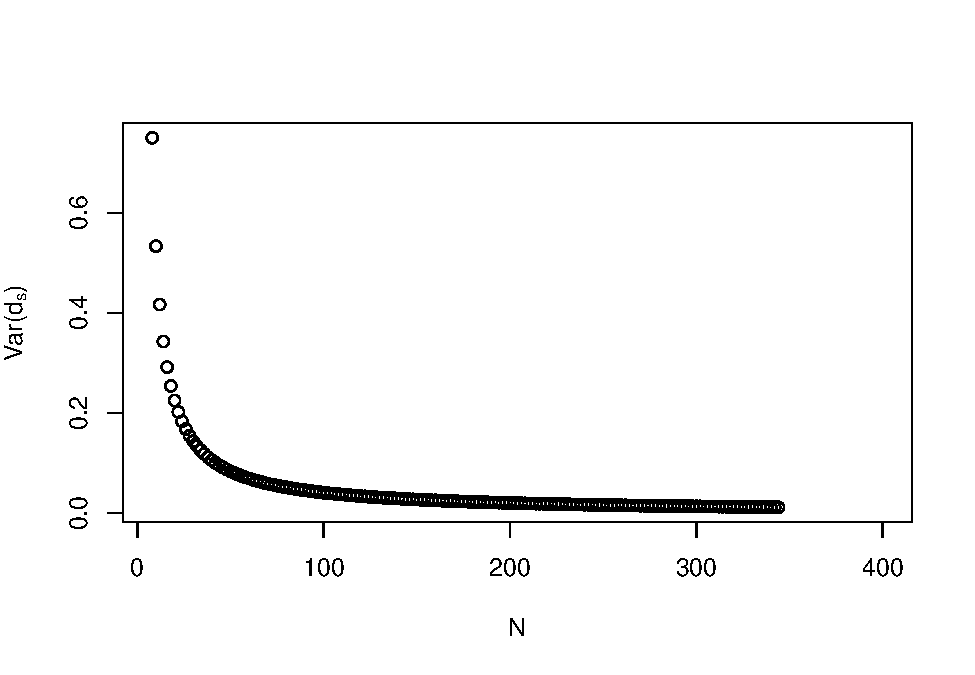
\includegraphics{Theoretical-Variance-of-all-estimators-as-a-function-of-population-parameters_files/figure-latex/varcohendNsize2-1.pdf}
\caption{\label{fig:varcohendNsize2}Variance of Cohen's \(d_s\), when variances are equal across groups, as a function of the total sample size (N).}
\end{figure}

\begin{itemize}
\tightlist
\item
  The larger the total sample size, the lower the variance. The variance tends to zero when the total sample size tends to infinity (see Figure \ref{fig:varcohendNsize2});
\end{itemize}

\begin{figure}
\centering
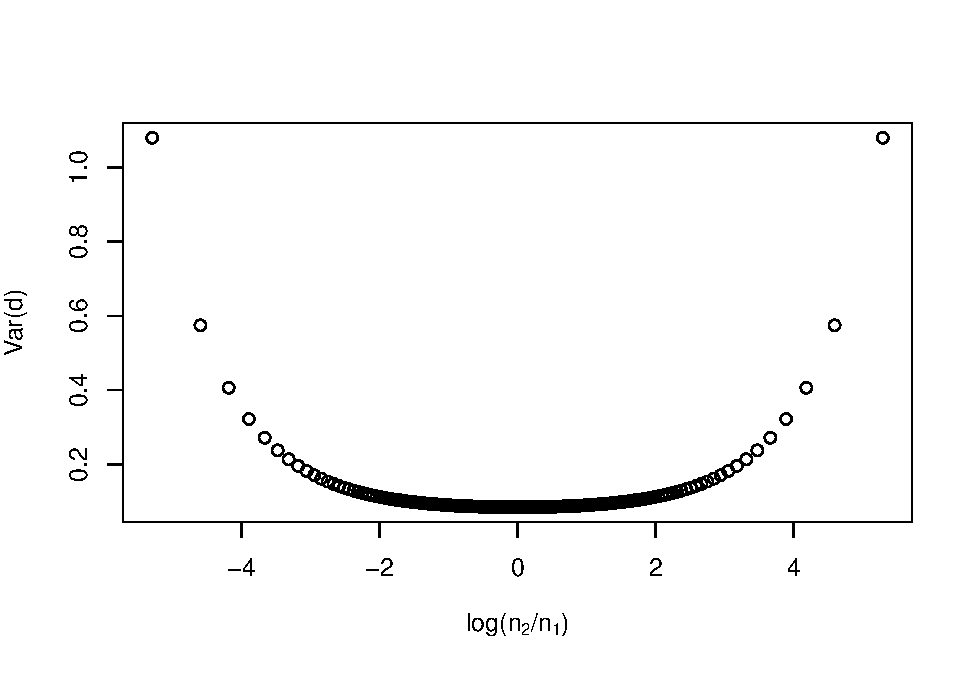
\includegraphics{Theoretical-Variance-of-all-estimators-as-a-function-of-population-parameters_files/figure-latex/varcohenNratio2-1.pdf}
\caption{\label{fig:varcohenNratio2}Variance of Cohen's \(d_s\), when variances are equal across groups, as a function of the logarithm of the sample sizes ratio (\(log\left(\frac{n_1}{n_2} \right)\)).}
\end{figure}

\begin{itemize}
\tightlist
\item
  The further the sample sizes allocation ratio is from 1, the larger the variance (see Figure \ref{fig:varcohenNratio2}).
\end{itemize}

\hypertarget{when-bf-pmbdelta_cohen-neq-0}{%
\paragraph{\texorpdfstring{When \(\bf \pmb{\delta_{Cohen}} \neq 0\)}{When \textbackslash bf \textbackslash pmb\{\textbackslash delta\_\{Cohen\}\} \textbackslash neq 0}}\label{when-bf-pmbdelta_cohen-neq-0}}

\begin{figure}
\centering
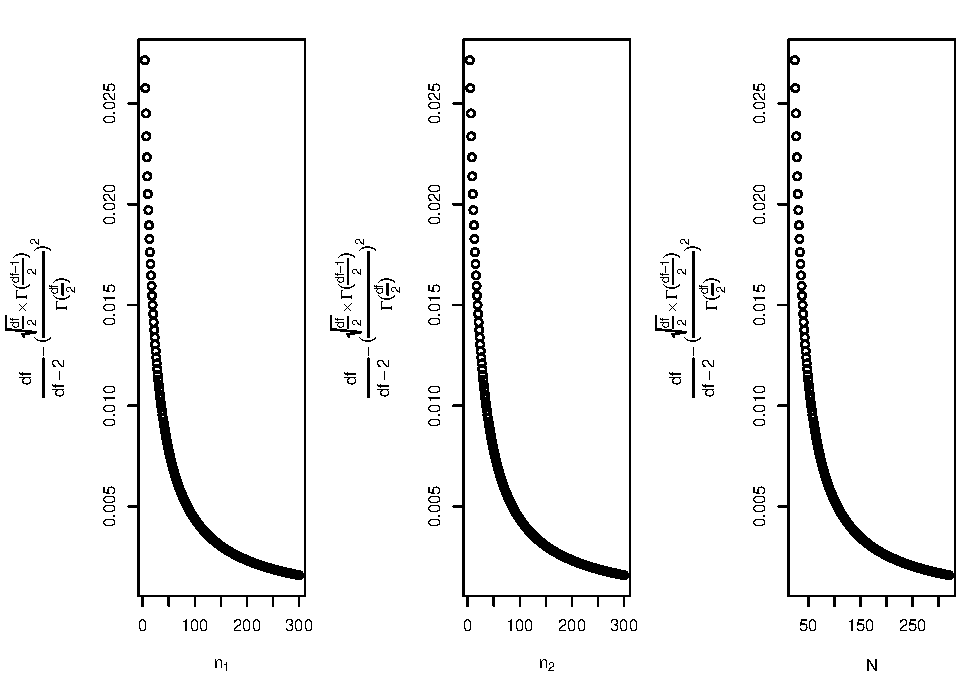
\includegraphics{Theoretical-Variance-of-all-estimators-as-a-function-of-population-parameters_files/figure-latex/ESmoderatorcohenNsize2-1.pdf}
\caption{\label{fig:ESmoderatorcohenNsize2}Effect size moderator, when computing the variance of Cohen's \(d_s\), as a function of \(n_1\) (left), \(n_2\) (center) and \(N=n_1+n_2\) (right).}
\end{figure}

While the variance of Cohen's \(d_s\) still depends on the total sample size and the sample sizes allocation ratio, it also depends on the population effect size (\(\delta_{Cohen}\)). The larger the population effect size, the larger the variance. Note that the effect of the population effect size decreases when sample sizes increase, as:\\
\[\lim_{n_1\rightarrow \infty}\left[\frac{df}{df-2} - \left( \frac{\sqrt{\frac{df}{2}} \times \Gamma \left(\frac{df-1}{2} \right)}{\Gamma \left( \frac{df}{2}\right)}\right)^2 \right]=0\]\\
\[\lim_{n_2\rightarrow \infty}\left[\frac{df}{df-2} - \left( \frac{\sqrt{\frac{df}{2}} \times \Gamma \left(\frac{df-1}{2} \right)}{\Gamma \left( \frac{df}{2}\right)}\right)^2 \right]=0\]\\
\[\lim_{N\rightarrow \infty}\left[\frac{df}{df-2} - \left( \frac{\sqrt{\frac{df}{2}} \times \Gamma \left(\frac{df-1}{2} \right)}{\Gamma \left( \frac{df}{2}\right)}\right)^2 \right]=0\]

This is illustrated in Figure \ref{fig:ESmoderatorcohenNsize2}.

\hypertarget{in-summary}{%
\subsubsection{In summary}\label{in-summary}}

The variance of Cohen's \(d_s\) is a function of the population effect size (\(\delta_{Cohen}\)), the total sample size (N) and the sample sizes ratio (\(\frac{n_1}{n_2}\)):

\begin{itemize}
\tightlist
\item
  The variance decreases when the total sample size increases;\\
\item
  The variance also decreases when the sample sizes ratio get closer to 1;\\
\item
  Finally, the variance increases when \(\delta_{Cohen}\) increases. Note that the effect of \(\delta_{Cohen}\) is moderated by the total sample size (the larger \(N\), the smaller the effect of \(\delta_{Cohen}\) on the variance).
\end{itemize}

\hypertarget{glasss-bf-d_s}{%
\subsection{\texorpdfstring{Glass's \(\bf d_s\)}{Glass's \textbackslash bf d\_s}}\label{glasss-bf-d_s}}

\hypertarget{when-variances-are-equal-across-populations-1}{%
\subsubsection{When variances are equal across populations}\label{when-variances-are-equal-across-populations-1}}

\hypertarget{when-bf-pmbdelta_glass0}{%
\paragraph{\texorpdfstring{When \(\bf \pmb{\delta_{Glass}}=0\)}{When \textbackslash bf \textbackslash pmb\{\textbackslash delta\_\{Glass\}\}=0}}\label{when-bf-pmbdelta_glass0}}

When the population effect size is zero, the variance of Glass's \(d_s\) can be simplified as follows:

\[Var_{Glass's \; d_s} = \frac{n_c-1}{n_c-3} \left( \frac{1}{n_c}+\frac{1}{n_e}\right)\]. In this configuration, the \textbf{variance} of Glass's \(d_s\) is a function of the sample sizes of both control (\(n_c\)) and experimental (\(n_e\)) groups as well as of the sample sizes allocation ratio \(\left( \frac{n_1}{n_2}\right)\):

\begin{figure}
\centering
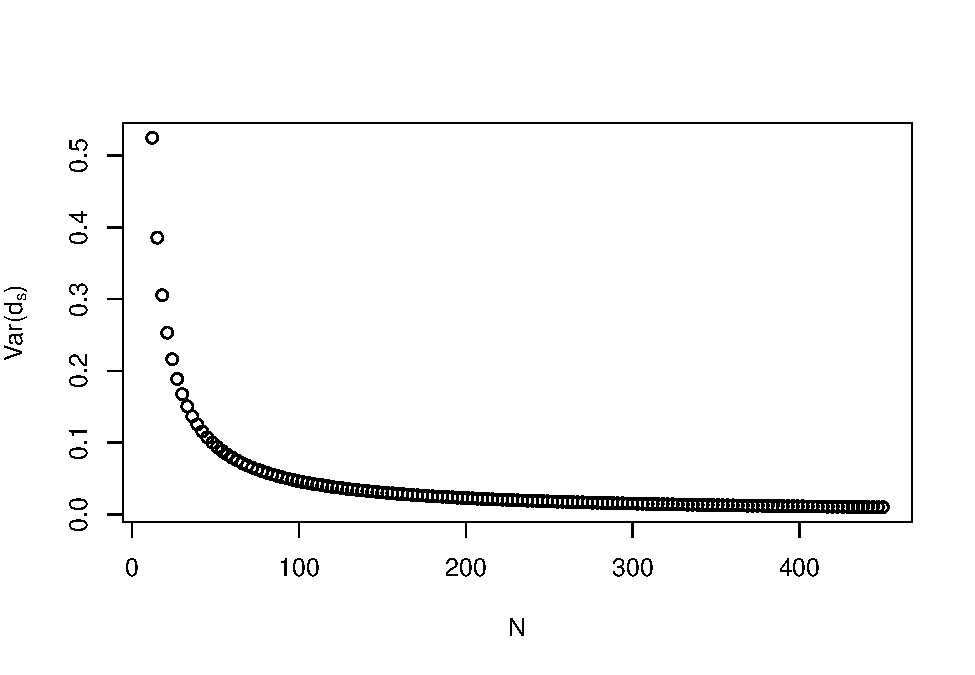
\includegraphics{Theoretical-Variance-of-all-estimators-as-a-function-of-population-parameters_files/figure-latex/varglassNsize2-1.pdf}
\caption{\label{fig:varglassNsize2}Variance of Glass's \(d_s\), when variances are equal across groups, as a function of the total sample size (N).}
\end{figure}

\begin{itemize}
\tightlist
\item
  The larger the sample sizes, the lower the variance (Figure \ref{fig:varglassNsize2});
\end{itemize}

\begin{figure}
\centering
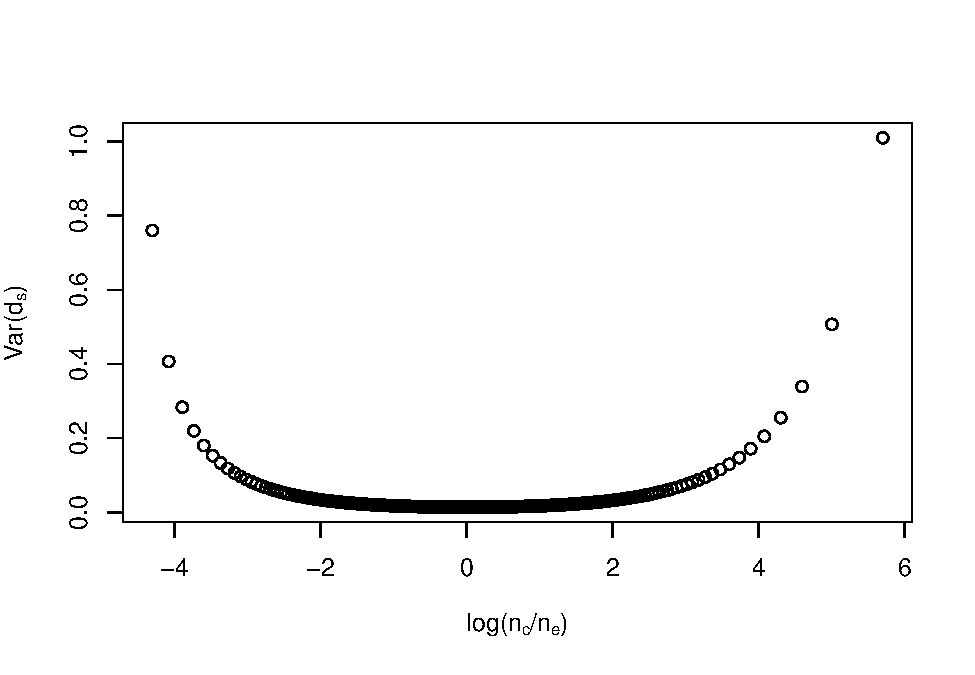
\includegraphics{Theoretical-Variance-of-all-estimators-as-a-function-of-population-parameters_files/figure-latex/varglasshomNratio2-1.pdf}
\caption{\label{fig:varglasshomNratio2}Variance of Glass's \(d_s\), when variances are equal across groups, as a function of the logarithm of the sample sizes ratio (\(log\left(\frac{n_c}{n_e} \right)\)).}
\end{figure}

The sample sizes ratio associated with the lowest variance is not exactly 1 (because of the term \(\frac{df}{df-2}\), df depending only on \(n_c\)), but is very close to 1 (and the larger the total sample size, the closer to 1 is the sample sizes ratio associated with the lowest variance). The further from this sample size ratio, the larger the variance (see Figure \ref{fig:varglasshomNratio2}).

\hypertarget{when-bf-pmbdelta_glass-neq-0}{%
\paragraph{\texorpdfstring{When \(\bf \pmb{\delta_{Glass}} \neq 0\)}{When \textbackslash bf \textbackslash pmb\{\textbackslash delta\_\{Glass\}\} \textbackslash neq 0}}\label{when-bf-pmbdelta_glass-neq-0}}

\begin{figure}
\centering
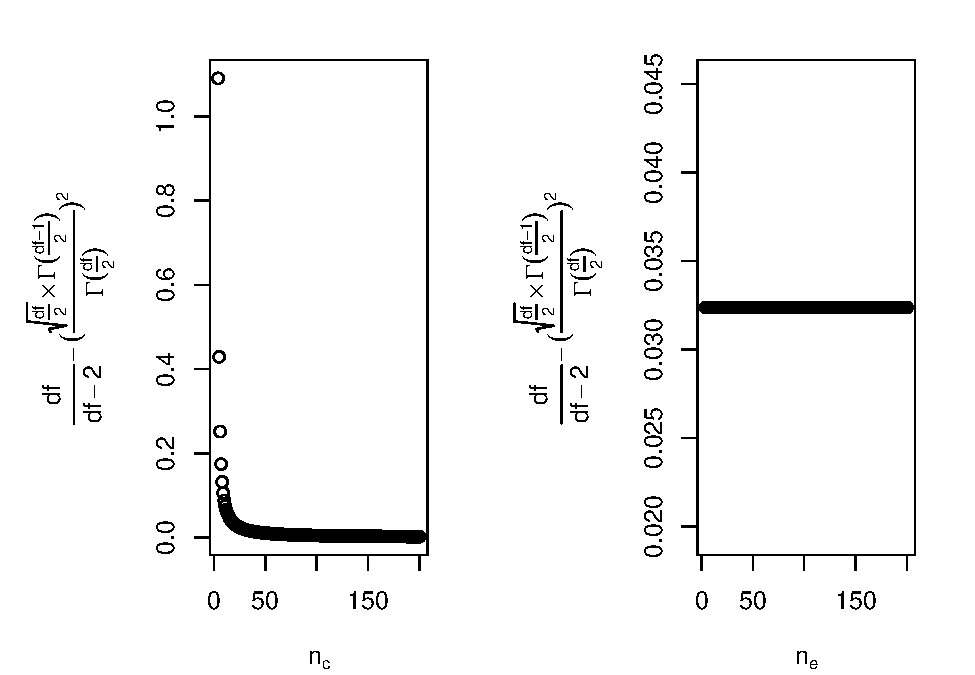
\includegraphics{Theoretical-Variance-of-all-estimators-as-a-function-of-population-parameters_files/figure-latex/ESmoderatorGlassNsize2-1.pdf}
\caption{\label{fig:ESmoderatorGlassNsize2}Effect size moderator, when computing the variance of Glass's \(d_s\), as a function of the size of the control group (left) and experimental group (right).}
\end{figure}

While the variance of Glass's \(d_s\) still depends on the total sample size and the sample sizes allocation ratio, it also depends on the population effect size (\(\delta_{Glass}\)). The larger the population effect size, the larger the variance. However, the effect of the population effect size decreases when the control group increases. On the other side, the effect of the population effect size does \emph{not} depend on the size of the experimental group.

\[\lim_{n_c\rightarrow \infty}\left[\frac{df}{df-2} - \left( \frac{\sqrt{\frac{df}{2}} \times \Gamma \left(\frac{df-1}{2} \right)}{\Gamma \left( \frac{df}{2}\right)}\right)^2 \right]=0\]
\[\lim_{n_e\rightarrow \infty}\left[\frac{df}{df-2} - \left( \frac{\sqrt{\frac{df}{2}} \times \Gamma \left(\frac{df-1}{2} \right)}{\Gamma \left( \frac{df}{2}\right)}\right)^2 \right] \neq 0\]

These limits are illustrated in Figure \ref{fig:ESmoderatorGlassNsize2}.

\begin{figure}
\centering
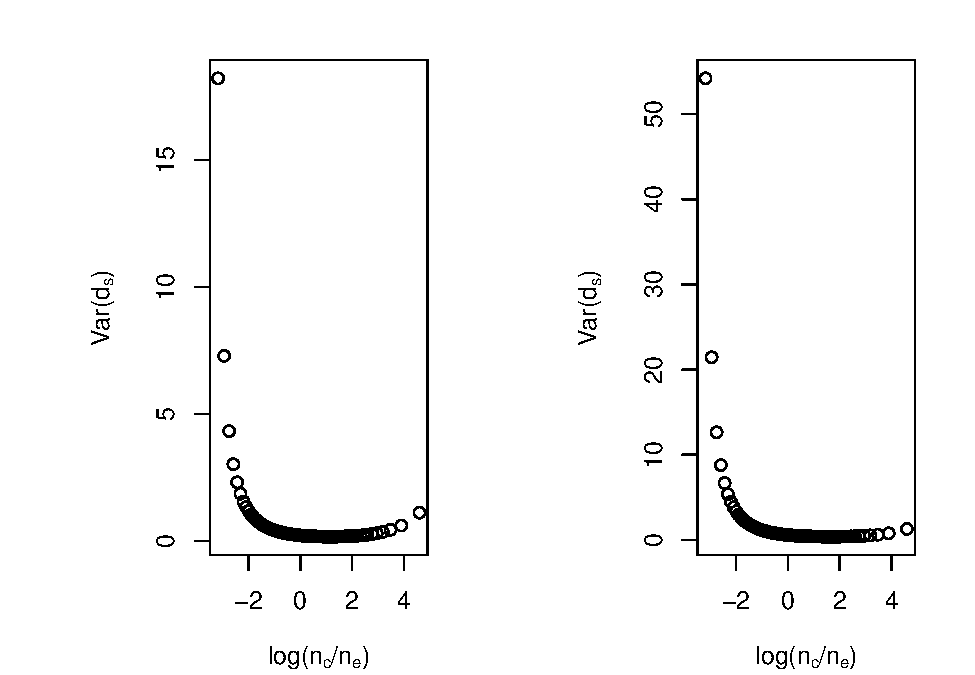
\includegraphics{Theoretical-Variance-of-all-estimators-as-a-function-of-population-parameters_files/figure-latex/varglasshomNratiobis2-1.pdf}
\caption{\label{fig:varglasshomNratiobis2}Variance of Glass's \(d_s\), when variances are equal across groups, as a function of the logarithm of the sample sizes ratio (\(log\left(\frac{n_c}{n_e} \right)\)) when \(\delta_{Glass}\) equals 4 (left) or 7 (right).}
\end{figure}

Note: while the sample sizes ratio associated with the lowest variance was very close to 1 with a null population effect size, this is not true anymore when the population effect size is not zero. Indeed, because of the second term in the adddition, when computing the variance, one gives much more weight to the effect size of the control group (see Figure \ref{fig:varglasshomNratiobis2}), and the larger the population effect size the truer. For example, when \(\delta_{Glass}\)= 4, the lowest variance will occur when \(n_c\) is approximately 3 times larger than \(n_e\). When \(\delta_{Glass}\)= 7, the lowest variance will occur when \(n_c\) is approximately 5 times larger than \(n_e\), etc.

\hypertarget{when-variances-are-unequal-across-populations-with-equal-sample-sizes}{%
\subsubsection{When variances are unequal across populations, with equal sample sizes}\label{when-variances-are-unequal-across-populations-with-equal-sample-sizes}}

\hypertarget{when-bf-pmbdelta_glass0-1}{%
\paragraph{\texorpdfstring{When \(\bf \pmb{\delta_{Glass}}=0\)}{When \textbackslash bf \textbackslash pmb\{\textbackslash delta\_\{Glass\}\}=0}}\label{when-bf-pmbdelta_glass0-1}}

When the population effect size is zero, the variance of Glass's \(d_s\) can be simplified as follows:

\[Var_{Glass's \; d_s} = \frac{n-1}{n(n-3)} \left( 1+\frac{\sigma^2_e}{\sigma^2_c}\right)\]
where \(n=N/2=\) sample size of each group. The variance is therefore a function of the total sample size and the \(SD\)-ratio (\(\frac{\sigma_c}{\sigma_e}\)):

\begin{figure}
\centering
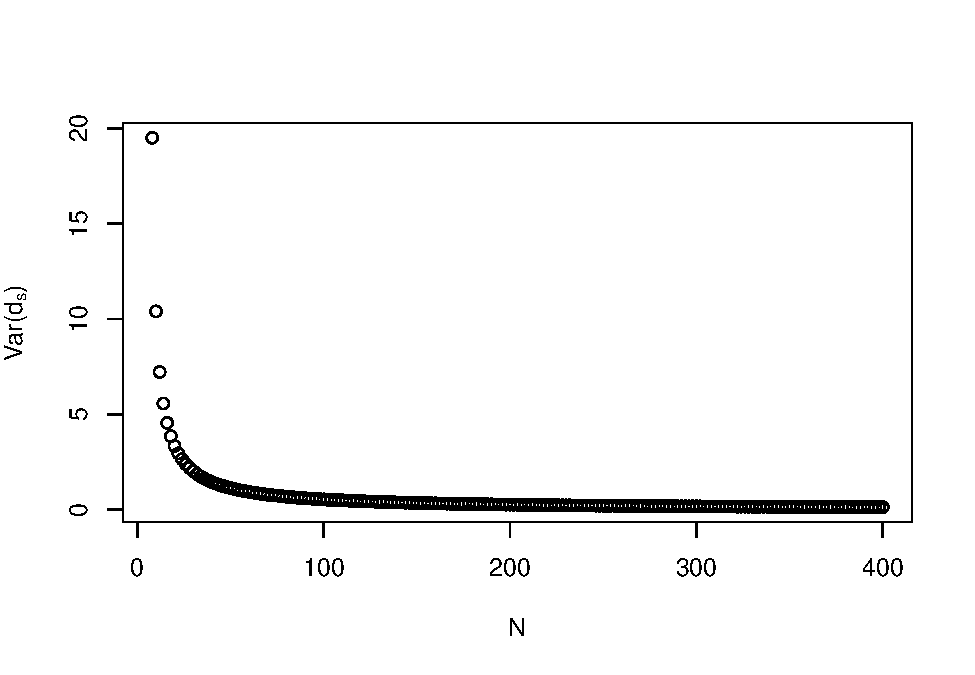
\includegraphics{Theoretical-Variance-of-all-estimators-as-a-function-of-population-parameters_files/figure-latex/varglassHetbalNsize2-1.pdf}
\caption{\label{fig:varglassHetbalNsize2}Variance of Glass's \(d_s\), when variances are unequal across groups and sample sizes are equal, as a function of the total sample sizes (N).}
\end{figure}

\begin{itemize}
\tightlist
\item
  The larger the total sample size, the lower the variance (See Figure \ref{fig:varglassHetbalNsize2});
\end{itemize}

\begin{figure}
\centering
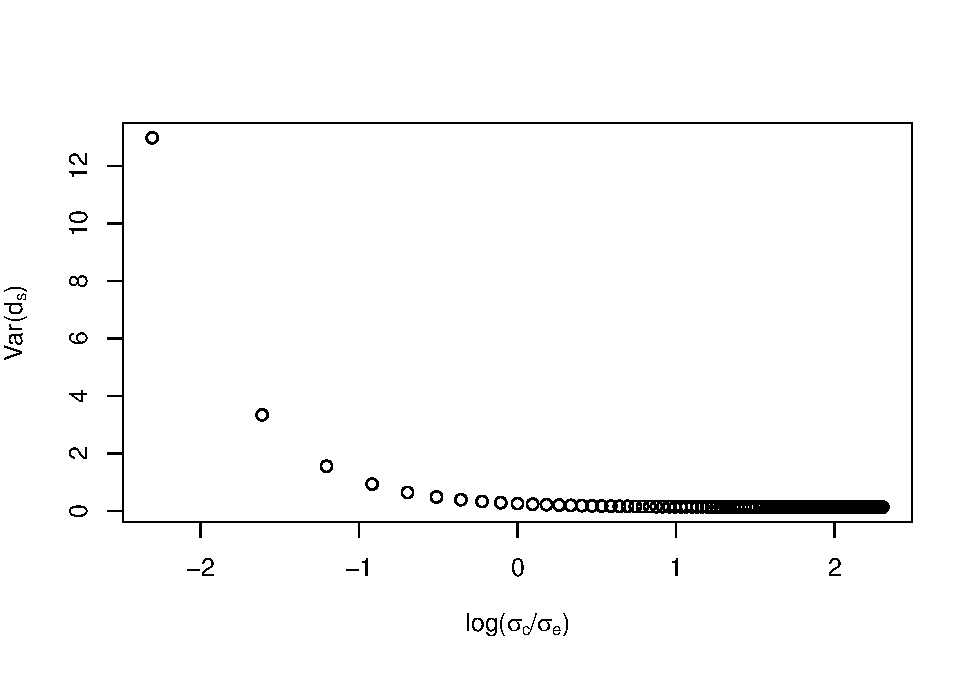
\includegraphics{Theoretical-Variance-of-all-estimators-as-a-function-of-population-parameters_files/figure-latex/varglasshetbalSDratio2-1.pdf}
\caption{\label{fig:varglasshetbalSDratio2}Variance of Glass's \(d_s\), when variances are unequal across groups and sample sizes are equal, as a function of the logarithm of the \(SD\)-ratio (\(log \left( \frac{\sigma_c}{\sigma_e} \right)\)).}
\end{figure}

\begin{itemize}
\tightlist
\item
  The larger the \(SD\)-ratio (i.e.~the larger is \(\sigma_c\) in comparison with \(\sigma_e\)), the lower the variance (see Figure \ref{fig:varglasshetbalSDratio2}). However, the effect of the \(SD\)-ratio decreases when sample sizes increase, because \(\lim_{n(=n_c=n_e)\rightarrow \infty}\left[\frac{df}{n(df-2)} \right]=0\).
\end{itemize}

\hypertarget{when-bf-pmbdelta_glass-neq-0-1}{%
\paragraph{\texorpdfstring{When \(\bf \pmb{\delta_{Glass}} \neq 0\)}{When \textbackslash bf \textbackslash pmb\{\textbackslash delta\_\{Glass\}\} \textbackslash neq 0}}\label{when-bf-pmbdelta_glass-neq-0-1}}

While the variance of Glass's \(d_s\) still depends on the total sample size and the \(SD\)-ratio, it also depends on the population effect size (\(\delta_{Glass}\)). The larger the population effect size, the larger the variance. However, the effect of the population effect size decreases when the control group increases, as previously explained and illustrated in Figure \ref{fig:ESmoderatorGlassNsize2}.

\hypertarget{when-variances-are-unequal-across-populations-with-unequal-sample-sizes}{%
\subsubsection{When variances are unequal across populations, with unequal sample sizes}\label{when-variances-are-unequal-across-populations-with-unequal-sample-sizes}}

\hypertarget{when-bf-pmbdelta_glass0-2}{%
\paragraph{\texorpdfstring{When \(\bf \pmb{\delta_{Glass}}=0\)}{When \textbackslash bf \textbackslash pmb\{\textbackslash delta\_\{Glass\}\}=0}}\label{when-bf-pmbdelta_glass0-2}}

When the population effect size is zero, the variance of Glass's \(d_s\) can be simplified as follows:

\[Var_{Glass's \; d_s} = \frac{n_c-1}{n_c-3} \left( \frac{1}{n_c}+\frac{\sigma^2_e}{n_e\sigma^2_c}\right)\]

The variance of Glass's \(d_s\) is therefore a function of the total sample size (N), the \(SD\)-ratio and the interaction between the sample sizes ratio and the \(SD\)-ratio \(\left(\frac{n_1}{n_2}\times\frac{\sigma_1}{\sigma_2} \right)\):

\begin{figure}
\centering
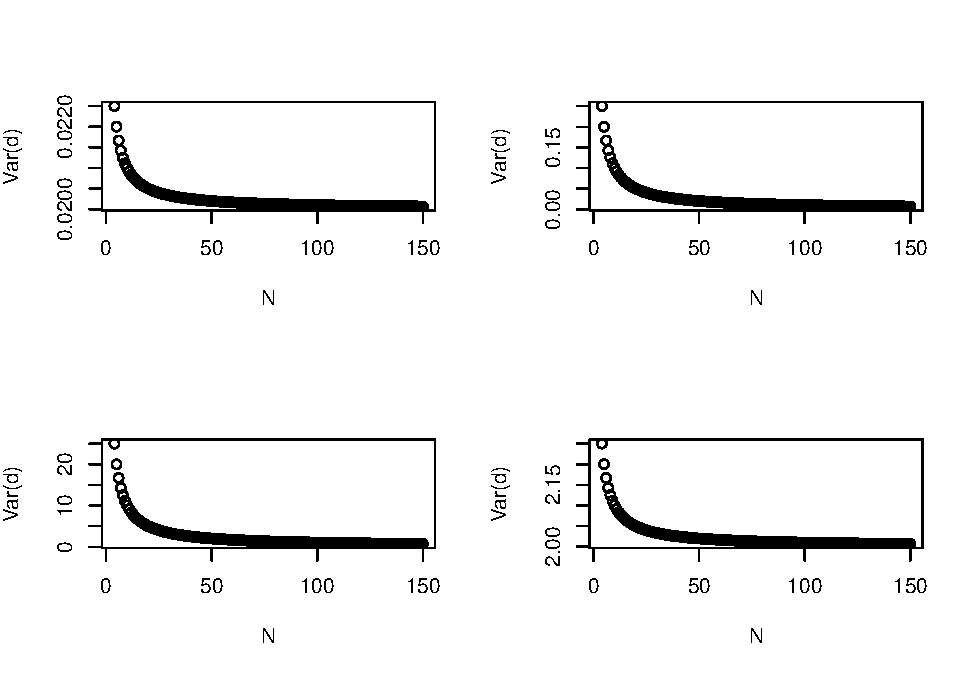
\includegraphics{Theoretical-Variance-of-all-estimators-as-a-function-of-population-parameters_files/figure-latex/varglassHetunbalNsize2-1.pdf}
\caption{\label{fig:varglassHetunbalNsize2}Variance of Glass's \(d_s\), when variances and sample sizes are unequal across groups, as a function of the total sample sizes, when increasing only the control (right) or the experimental (left) group, when \(\sigma_c > \sigma_e\) (top plots) or \(\sigma_c < \sigma_e\) (bottom plots).}
\end{figure}

\begin{itemize}
\item
  Whatever the \(SD\) and sample sizes pairing, increasing \(n_c\) and/or \(n_e\) will decrease the variance (see Figure \ref{fig:varglassHetunbalNsize2});

  \begin{itemize}
  \tightlist
  \item
    The effect of the sample sizes ratio depends on the \(SD\)-ratio:

    \begin{itemize}
    \tightlist
    \item
      We previously mentioned that when \(\sigma_c=\sigma_e\), the variance is minimized when sample sizes of both groups are almost identical (see Figure \ref{fig:varglasshomNratio2}), meaning that it is more efficient, in order to reduce variance, to add subjects uniformly in both groups;\\
    \item
      When \(\sigma_e > \sigma_c\), more weight is given to \(n_e\), meaning that it is more efficient, in order to reduce variance, to add subjects in the experimental group (\(n_e\); see bottom plots in Figure \ref{fig:varglassHetunbalNsize2});\\
    \item
      When \(\sigma_c > \sigma_e\), less weight is given to \(n_e\), meaning that it is more efficient, in order to reduce variance, to add sujects in the control group (\(n_c\); see top plots in Figure \ref{fig:varglassHetunbalNsize2}).
    \end{itemize}
  \end{itemize}
\end{itemize}

\begin{figure}
\centering
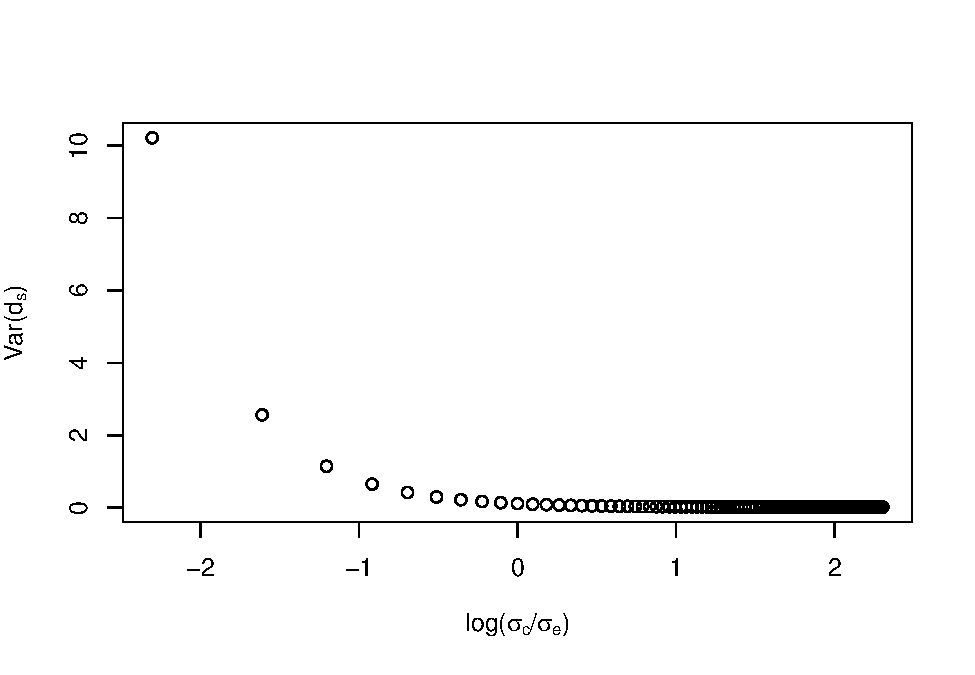
\includegraphics{Theoretical-Variance-of-all-estimators-as-a-function-of-population-parameters_files/figure-latex/varglasshetunbalSDratio2-1.pdf}
\caption{\label{fig:varglasshetunbalSDratio2}Variance of Glass's \(d_s\), when sample sizes and variances are unequal across groups, as a function of the logarithm of the \(SD\)-ratio (\(log \left( \frac{\sigma_c}{\sigma_e} \right)\)).}
\end{figure}

\begin{itemize}
\tightlist
\item
  Finally, there is also a main effect of the \(SD\)-ratio: the larger is \(\sigma_c\) in comparison with \(\sigma_e\), the lower the variance, as we can observe in Figure \ref{fig:varglasshetunbalSDratio2}. We can also notice that in Figure \ref{fig:varglassHetunbalNsize2}, the maximum variance is much larger in the two bottom plots (where \(\sigma_c<\sigma_e\)) than in the two top plots (where \(\sigma_c>\sigma_e\)).
\end{itemize}

Note that the effect of the \(SD\)-ratio, and the interaction effect between \(SD\)-ratio and sample sizes ratio decreases when the sample size of the control group increases (because \(\frac{n_c-1}{n_c-3}\) get closer to 1).

\hypertarget{when-bf-pmbdelta_glass-neq-0-2}{%
\paragraph{\texorpdfstring{When \(\bf \pmb{\delta_{Glass}} \neq 0\)}{When \textbackslash bf \textbackslash pmb\{\textbackslash delta\_\{Glass\}\} \textbackslash neq 0}}\label{when-bf-pmbdelta_glass-neq-0-2}}

While the variance of Glass's \(d_s\) still depends on the total sample size, the \(SD\)-ratio and the interaction between the \(SD\)-ratio and the sample sizes ratio, it also depends on the population effect size (\(\delta_{Glass}\)): the larger the population effect size, the larger the variance. However, the effect of the population effect size decreases when the sample size of the control group increases, as previously explained and illustrated in Figure \ref{fig:ESmoderatorGlassNsize2}.

Note: when the population effect size was null, when \(\sigma_c<\sigma_e\), it was much more efficient to add subjects in the experimental group in order to reduce the variance (because much more weight were given to \(n_e\)). When \(\delta_{Glass} \neq 0\), it is important to add subjects in both groups in order to reduce the variance (because \(\frac{df}{df-2} - \left( \frac{\sqrt{\frac{df}{2}} \times \Gamma \left(\frac{df-1}{2} \right)}{\Gamma \left( \frac{df}{2}\right)}\right)^2\) is only a function of the sample size of the control group). With huge population effect size, it is even always more important to add subjects in the control group (e.g.~when \(\delta_{Glass}=30\)).

\hypertarget{in-summary-1}{%
\subsubsection{In summary}\label{in-summary-1}}

The variance of Glass's \(d_s\) is a function of the population effect size (\(\delta_{Glass}\)), the \(SD\)-ratio, the total sample size and the interaction between sample sizes ratio and \(SD\)-ratio \(\left(\frac{n_1}{n_2}\times\frac{\sigma_1}{\sigma_2} \right)\):

\begin{itemize}
\tightlist
\item
  The variance decreases when the \(SD\)-ratio increases (i.e.~when \(\sigma_e >> \sigma_c\));\\
\item
  The variance always decreases when the control and/or the experimental group increases. The benefit of adding subjects rather in the control, in the experimental, or in both groups, in order to reduce the variance, varies as a function of the \(SD\)-ratio and the population effect size. The only situation where it is optimal to maximize the experimental group is when \(\sigma_e > \sigma_c\) and \(\sigma_{Glass} \approx 0\). Most of the time, it is more efficient to maximize the control groups (e.g.~anytime \(\sigma_e < \sigma_c\), and when \(\sigma_{Glass}\) is very large) or to uniformly add subjects in both groups (e.g.~when \(\sigma_e > \sigma_c\) and \(\delta_{Glass}\) is neither null nor huge);
\item
  The variance increases when \(\delta_{Glass}\) increases. Note that the effect of \(\delta_{Glass}\) is moderated by the control group size (the larger \(n_e\), the smaller the effect of \(\delta_{Glass}\) on the variance).
\end{itemize}

\hypertarget{cohens-bf-d_s-1}{%
\subsection{\texorpdfstring{Cohen's \(\bf d^*_s\)}{Cohen's \textbackslash bf d\^{}*\_s}}\label{cohens-bf-d_s-1}}

\hypertarget{when-variances-are-equal-across-populations-2}{%
\subsubsection{When variances are equal across populations}\label{when-variances-are-equal-across-populations-2}}

\hypertarget{when-bf-pmbdelta_cohen0-1}{%
\paragraph{\texorpdfstring{When \(\bf \pmb{\delta^*_{Cohen}}=0\)}{When \textbackslash bf \textbackslash pmb\{\textbackslash delta\^{}*\_\{Cohen\}\}=0}}\label{when-bf-pmbdelta_cohen0-1}}

When the population effect size is zero, the variance of Cohen's \(d^*_s\) is computed as following :

\[var_{Cohen's \; d^*_s} = \frac{df}{df-2} \times \frac{N}{n_1n_2}\]
with \[df = \frac{4(n_1-1)(n_2-1)}{n_1+n_2-2}\]

In this configuration, the degrees of freedom as well as the variance of Cohen's \(d^*_s\) depends on the total sample size (N) and the sample sizes allocation ratio (\(\frac{n_1}{n_2}\)):

\begin{figure}
\centering
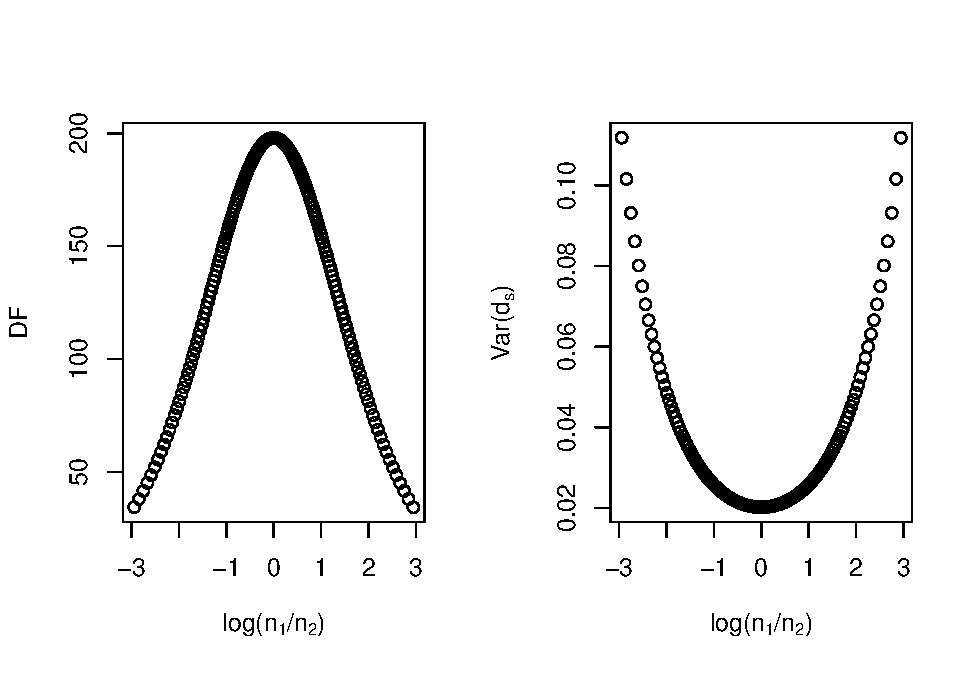
\includegraphics{Theoretical-Variance-of-all-estimators-as-a-function-of-population-parameters_files/figure-latex/varcohendprimeHomNratio2-1.pdf}
\caption{\label{fig:varcohendprimeHomNratio2}Variance of Cohen's \(d^*_s\) when variances are equal across groups, as a function of the logarithm of the sample sizes ratio (\(log\left(\frac{n_1}{n_2} \right)\)).}
\end{figure}

\begin{itemize}
\tightlist
\item
  The further the sample sizes allocation ratio is from 1, the larger the variance (see Figure \ref{fig:varcohendprimeHomNratio2});
\end{itemize}

\begin{figure}
\centering
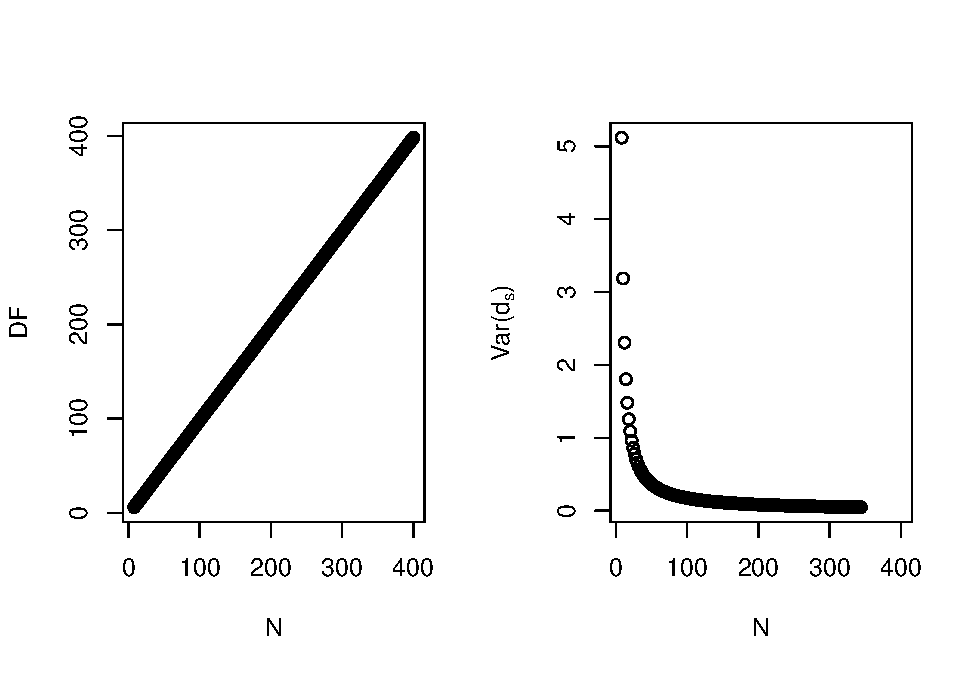
\includegraphics{Theoretical-Variance-of-all-estimators-as-a-function-of-population-parameters_files/figure-latex/varcohendprimehomNsize2-1.pdf}
\caption{\label{fig:varcohendprimehomNsize2}Variance of Cohen's \(d^*_s\) when variances are equal across groups, as a function of the total sample size (N).}
\end{figure}

\begin{itemize}
\tightlist
\item
  The larger the total sample size, the lower the bias (see Figure \ref{fig:varcohendprimehomNsize2}).
\end{itemize}

\hypertarget{when-bf-pmbdelta_cohen-neq-0-1}{%
\paragraph{\texorpdfstring{When \(\bf \pmb{\delta^*_{Cohen}} \neq 0\)}{When \textbackslash bf \textbackslash pmb\{\textbackslash delta\^{}*\_\{Cohen\}\} \textbackslash neq 0}}\label{when-bf-pmbdelta_cohen-neq-0-1}}

\begin{figure}
\centering
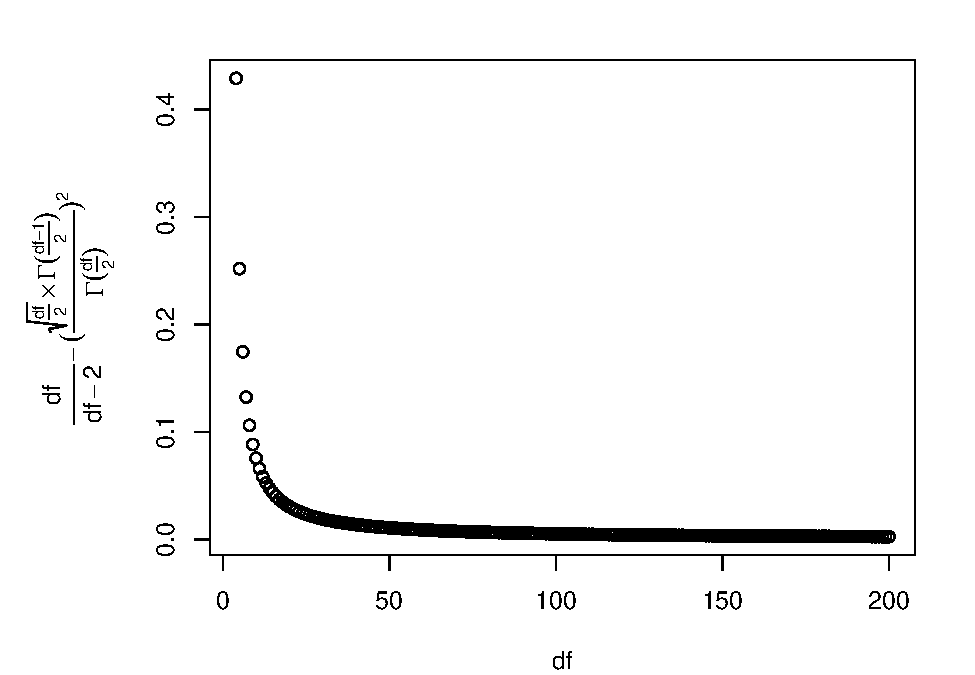
\includegraphics{Theoretical-Variance-of-all-estimators-as-a-function-of-population-parameters_files/figure-latex/ESmoderator2-1.pdf}
\caption{\label{fig:ESmoderator2}Effect size moderator, as a function of the degrees of freedom.}
\end{figure}

While the variance of Cohen's \(d^*_s\) still depends on the total sample size and the sample sizes ratio, it also depends on the population effect size (\(\delta^*_{Cohen}\)): the larger the population effect size, the larger the variance. However, the effect of the population effect size decreases when the degrees of freedom increase (i.e.~when sample sizes increase and/or the sample sizes ratio get closer to 1), as illustrated in Figure \ref{fig:ESmoderator2}:

\[\lim_{df\rightarrow \infty}\left[\frac{df}{df-2} - \left( \frac{\sqrt{\frac{df}{2}} \times \Gamma \left(\frac{df-1}{2} \right)}{\Gamma \left( \frac{df}{2}\right)}\right)^2 \right]=0\]

\hypertarget{when-variances-are-unequal-across-populations-with-equal-sample-sizes-1}{%
\subsubsection{When variances are unequal across populations, with equal sample sizes}\label{when-variances-are-unequal-across-populations-with-equal-sample-sizes-1}}

\hypertarget{when-bf-pmbdelta_cohen0-2}{%
\paragraph{\texorpdfstring{When \(\bf \pmb{\delta^*_{Cohen}}=0\)}{When \textbackslash bf \textbackslash pmb\{\textbackslash delta\^{}*\_\{Cohen\}\}=0}}\label{when-bf-pmbdelta_cohen0-2}}

When the population effect size is zero, the variance of Cohen's \(d^*_s\) can be simplified as follows:

\[var_{Cohen's \; d^*_s} = \frac{df}{df-2} \times \frac{2}{n}\]
Where \(n=N/2\)=sample size of each group, and \(df=\frac{(n-1)(\sigma^4_1+\sigma^4_2+2\sigma^2_1\sigma^2_2)}{\sigma^4_1+\sigma^4_2}\). In this configuration, the degrees of freedom as well as the variance of Cohen's \(d_s\) depends on the total sample size (N) and the \(SD\)-ratio \(\left( \frac{\sigma_1}{\sigma_2}\right)\):

\begin{figure}
\centering
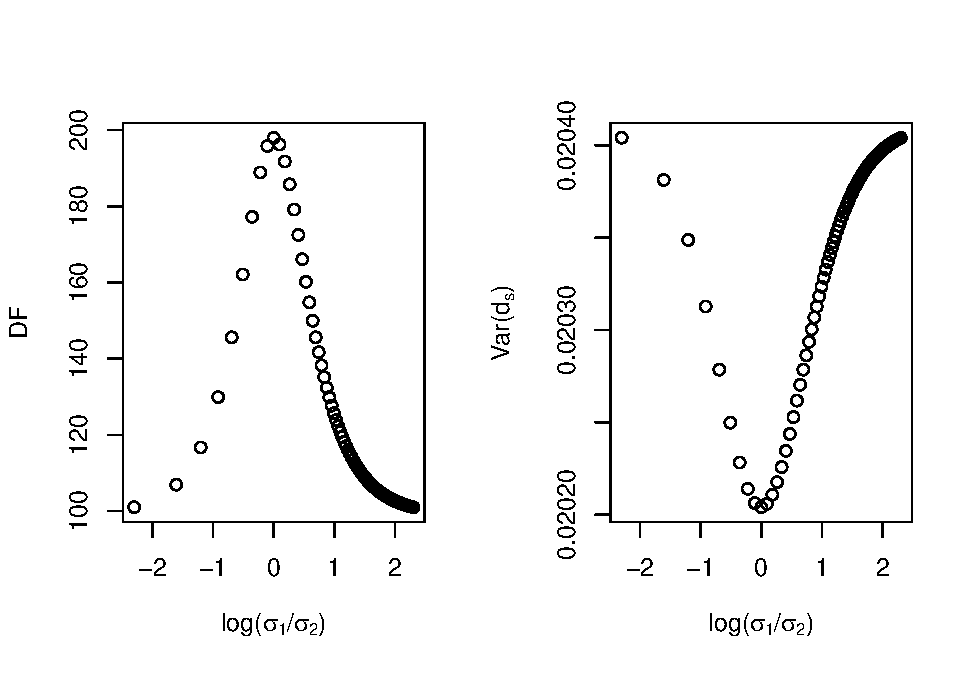
\includegraphics{Theoretical-Variance-of-all-estimators-as-a-function-of-population-parameters_files/figure-latex/varcohendprimehetbalSDratio2-1.pdf}
\caption{\label{fig:varcohendprimehetbalSDratio2}Variance of Cohen's \(d^*_s\) when variances are unequal across groups and sample sizes are equal, as a function of the logarithm of the \(SD\)-ratio (\(log \left( \frac{\sigma_1}{\sigma_2} \right)\)).}
\end{figure}

\begin{itemize}
\tightlist
\item
  The further the \(SD\)-ratio is from 1, the larger the variance (see Figure \ref{fig:varcohendprimehetbalSDratio2});
\end{itemize}

\begin{figure}
\centering
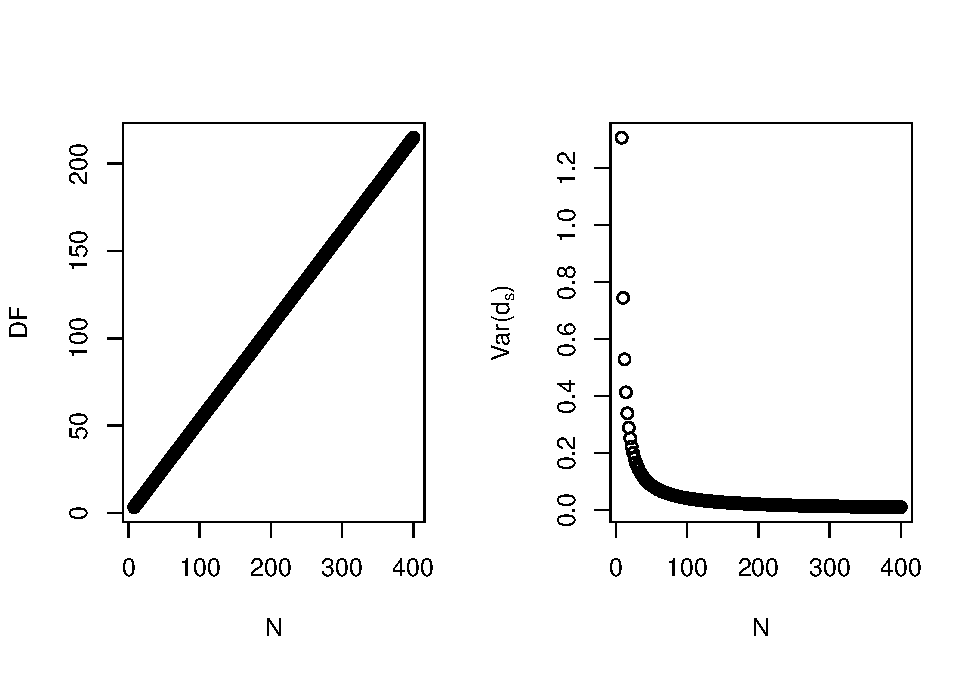
\includegraphics{Theoretical-Variance-of-all-estimators-as-a-function-of-population-parameters_files/figure-latex/varcohendprimehetbalNsize2-1.pdf}
\caption{\label{fig:varcohendprimehetbalNsize2}Variance of Cohen's \(d^*_s\) when variances are unequal across groups and sample sizes are equal, as a function of the total sample size (N).}
\end{figure}

\begin{itemize}
\tightlist
\item
  The larger the total sample size, the lower the variance (see Figure \ref{fig:varcohendprimehetbalNsize2}).
\end{itemize}

\begin{figure}
\centering
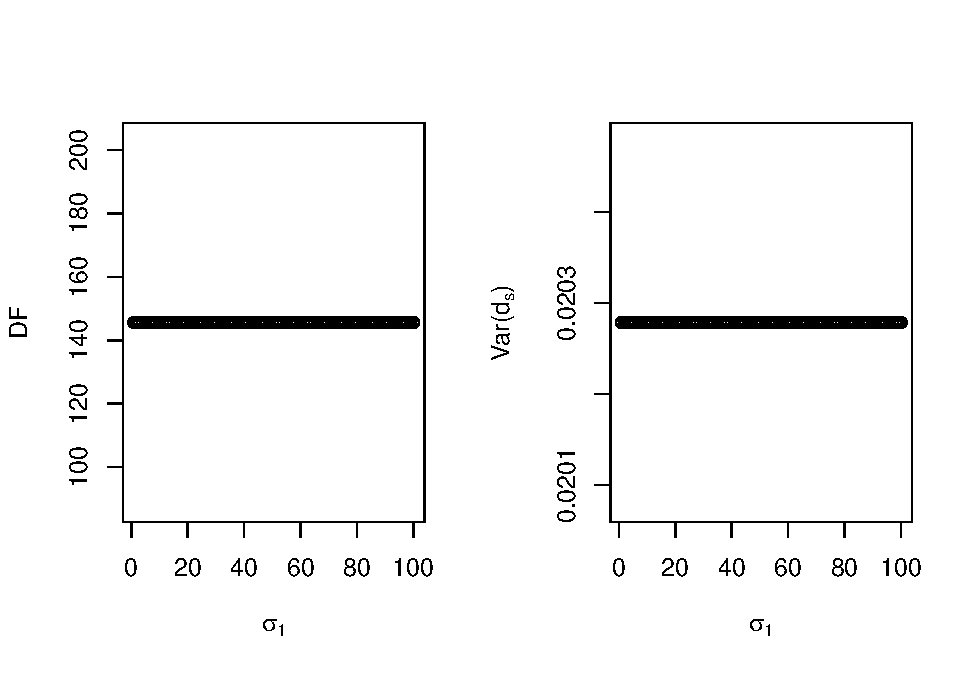
\includegraphics{Theoretical-Variance-of-all-estimators-as-a-function-of-population-parameters_files/figure-latex/varcohendprimehetbalvariance2-1.pdf}
\caption{\label{fig:varcohendprimehetbalvariance2}Variance of Cohen's \(d^*_s\), when variances are unequal across groups and sample sizes are equal, as a function of \(\sigma_1\) and \(\sigma_2\), for a constant \(SD\)-ratio.}
\end{figure}

Note: for a constant \(SD\)-ratio, the size of the variance does not matter (see Figure \ref{fig:varcohendprimehetbalvariance2}).

\hypertarget{when-bf-pmbdelta_cohen-neq-0-2}{%
\paragraph{\texorpdfstring{When \(\bf \pmb{\delta^*_{Cohen}} \neq 0\)}{When \textbackslash bf \textbackslash pmb\{\textbackslash delta\^{}*\_\{Cohen\}\} \textbackslash neq 0}}\label{when-bf-pmbdelta_cohen-neq-0-2}}

While the variance of Cohen's \(d^*_s\) still depednds on the total sample size and the \(SD\)-ratio, it also depends on the population effect size (\(\delta^*_{Cohen}\)): the larger the population effect size, the larger the variance. However, the effect of the population effect size decreases when the degrees of freedom increase (i.e.~when the total sample size increases and/or the \(SD\)-ratio get closer to 1), as previously illustrated in Figure \ref{fig:ESmoderator2}.

\hypertarget{when-variances-are-unequal-across-populations-with-unequal-sample-sizes-1}{%
\subsubsection{When variances are unequal across populations, with unequal sample sizes}\label{when-variances-are-unequal-across-populations-with-unequal-sample-sizes-1}}

\hypertarget{when-bf-pmbdelta_cohen0-3}{%
\paragraph{\texorpdfstring{When \(\bf \pmb{\delta^*_{Cohen}}=0\)}{When \textbackslash bf \textbackslash pmb\{\textbackslash delta\^{}*\_\{Cohen\}\}=0}}\label{when-bf-pmbdelta_cohen0-3}}

When the population effect size is zero, the variance of Cohen's \(d^*_s\) can be simplified as follows:

\[Var_{Cohen's \; d^*_s} = \frac{df}{df-2} \times \frac{2\left( \frac{\sigma^2_1}{n_1} + \frac{\sigma^2_2}{n_2} \right)}{\sigma^2_1+\sigma^2_2}\]
with \(df =\frac{(n_1-1)(n_2-1)(\sigma^2_1+\sigma^2_2)^2}{(n_2-1)\sigma_1^4+(n_1-1)\sigma_2^4}\). In this configuration, the degrees of freedom are a function of the total sample size (N) and the interaction between sample sizes ratio and the \(SD\)-ratio \(\left(\frac{n_1}{n_2}\times\frac{\sigma_1}{\sigma_2} \right)\):

\begin{figure}
\centering
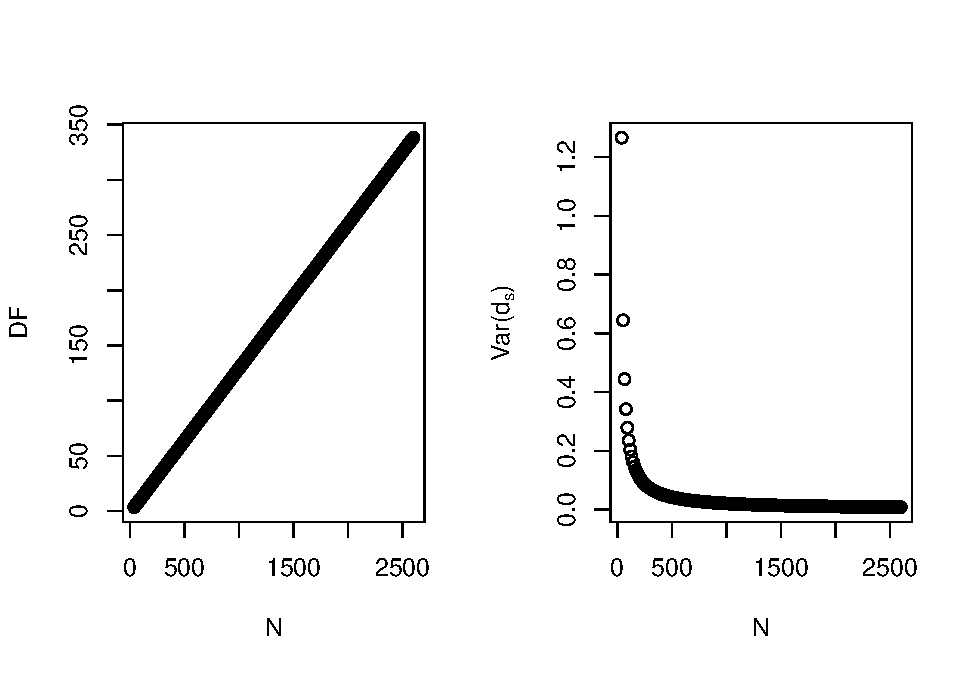
\includegraphics{Theoretical-Variance-of-all-estimators-as-a-function-of-population-parameters_files/figure-latex/varcohendprimehetunbalNsize2-1.pdf}
\caption{\label{fig:varcohendprimehetunbalNsize2}Variance of Cohen's \(d^*_s\) when variances and sample sizes are unequal across groups, as a function of the total sample size (N).}
\end{figure}

\begin{itemize}
\tightlist
\item
  The larger the total sample size, the lower the variance (illustration in Figure \ref{fig:varcohendprimehetunbalNsize2});
\end{itemize}

\begin{figure}
\centering
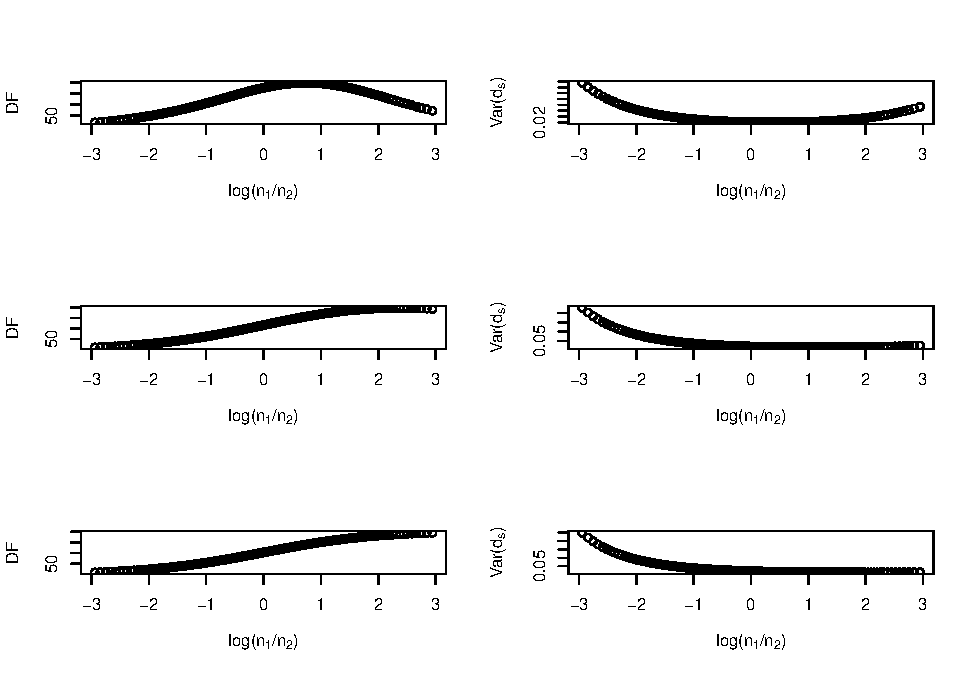
\includegraphics{Theoretical-Variance-of-all-estimators-as-a-function-of-population-parameters_files/figure-latex/varcohendprimehetunbalnratiosdratio2-1.pdf}
\caption{\label{fig:varcohendprimehetunbalnratiosdratio2}The variance of Cohen's \(d^*_s\), when variances and sample sizes are unequal across groups, as a function of the logarithm of the sample sizes ratio (\(log \left( \frac{n_1}{n_2} \right)\)), when \(SD\)-ratio equals 1.46 (first row), 3.39 (second row) or 7 (third row).}
\end{figure}

\begin{itemize}
\tightlist
\item
  The smallest variance always occurs when there is a positive pairing between variances and sample sizes, because one gives more weight to the smallest variance in the denominator of the df computation and in the numerator of the variance computation. Moreover, the further the \(SD\)-ratio is from 1, the further from 1 will also be the sample sizes ratio associated with the smallest variance (see Figure \ref{fig:varcohendprimehetunbalnratiosdratio2}). This can be explained by splitting the numerator and the denominator of the DF computation (see the file \enquote{Theoretical Bias, as a function of population parameters}).
\end{itemize}

\begin{figure}
\centering
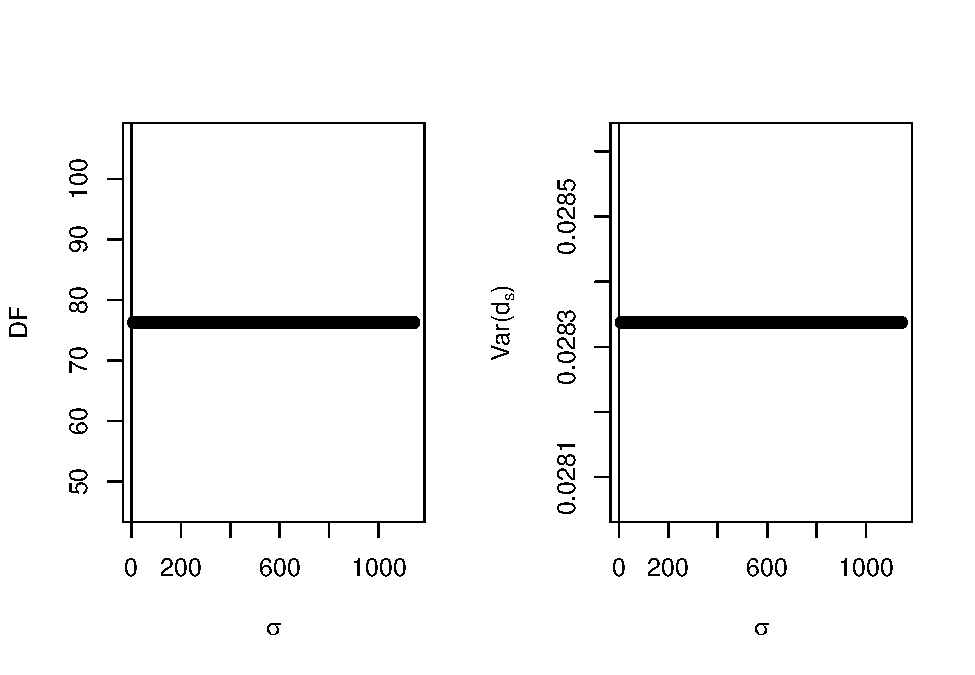
\includegraphics{Theoretical-Variance-of-all-estimators-as-a-function-of-population-parameters_files/figure-latex/varcohendprimehetunbalvariance2-1.pdf}
\caption{\label{fig:varcohendprimehetunbalvariance2}Variance of Cohen's \(d^*_s\), when variances and sample sizes are unequal across groups, as a function of \(\sigma_1\) and \(\sigma_2\), for a constant \(SD\)-ratio.}
\end{figure}

Note: for a constant SD-ratio, the variance does not matter. (See Figure \ref{fig:varcohendprimehetunbalvariance2}).

\hypertarget{when-bf-pmbdelta_cohen-neq-0-3}{%
\paragraph{\texorpdfstring{When \(\bf \pmb{\delta^*_{Cohen}} \neq 0\)}{When \textbackslash bf \textbackslash pmb\{\textbackslash delta\^{}*\_\{Cohen\}\} \textbackslash neq 0}}\label{when-bf-pmbdelta_cohen-neq-0-3}}

While the variance of Cohen's \(d^*_s\) still depends on the total sample size, the \(SD\)-ratio and the interaction between the sample sizes ratio and the \(SD\)-ratio, it also depends on the population effect size (\(\delta^*_{Cohen}\)): the larger the population effect size, the larger the variance. However, the effect of the population effect size decreases when the degrees of freedom increase (i.e.~when the total sample size increases and/or when there is a positive pairing between the sample sizes ratio and the \(SD\)-ratio), as previously illustrated in Figure \ref{fig:ESmoderator2}.

\hypertarget{in-summary-2}{%
\subsubsection{In summary}\label{in-summary-2}}

The variance of Cohen's \(d^*_s\) is a function of the population effect size (\(\delta^*_{Cohen}\)), the total sample size (N) and the interaction between sample sizes ratio and \(SD\)-ratio \(\left(\frac{n_1}{n_2}\times\frac{\sigma_1}{\sigma_2} \right)\):

\begin{itemize}
\tightlist
\item
  The variance always decreases when the control and/or the experimental group increases. The benefit of adding subjects rather in the control or in the experimental group depends on the \(SD\)-ratio. Indeed, the smallest variance always occurs when there is a positive pairing between variances and sample sizes. Moreover, the further the \(SD\)-ratio is from 1, the further from 1 will also be the sample sizes ratio associated with the smallest variance;\\
\item
  The variance increases when \(\delta^*_{Cohen}\) increases. Note that the effect of \(\delta^*_{Cohen}\) is moderated by the total sample size and the interaction between sample sizes ratio and \(SD\)-ratio.
\end{itemize}

\hypertarget{shiehs-bf-d_s}{%
\subsection{\texorpdfstring{Shieh's \(\bf d_s\)}{Shieh's \textbackslash bf d\_s}}\label{shiehs-bf-d_s}}

\hypertarget{when-variances-are-equal-across-populations-3}{%
\subsubsection{When variances are equal across populations}\label{when-variances-are-equal-across-populations-3}}

\hypertarget{when-bf-pmbdelta_shieh0}{%
\paragraph{\texorpdfstring{When \(\bf \pmb{\delta_{Shieh}}=0\)}{When \textbackslash bf \textbackslash pmb\{\textbackslash delta\_\{Shieh\}\}=0}}\label{when-bf-pmbdelta_shieh0}}

When the population effect size is zero, the variance of Shieh's \(d_s\) can be simplified as follows:

\[Var_{Shieh's \; d_s} = \frac{df}{(df-2)N}\]
with \(df = \frac{N^2(n_1-1)(n_2-1)}{n_2^2(n_2-1)+n_1^2(n_1-1)}\). In this configuration, the degrees of freedom as well as the variance of Shieh's \(d_s\) depend on the total sample size (N) and the sample sizes allocation ratio (\(\frac{n_1}{n_2}\)):

\begin{figure}
\centering
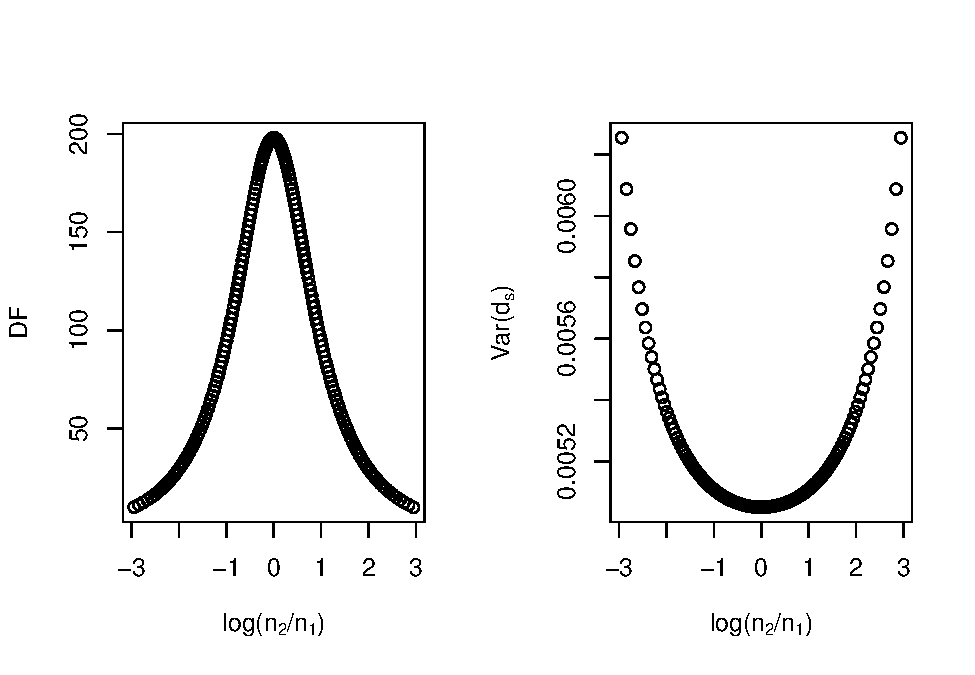
\includegraphics{Theoretical-Variance-of-all-estimators-as-a-function-of-population-parameters_files/figure-latex/varshiehHomNratio2-1.pdf}
\caption{\label{fig:varshiehHomNratio2}Variance of Shieh's \(d_s\) when variances are equal across groups, as a function of the logarithm of the sample sizes ratio (\(log\left(\frac{n_1}{n_2} \right)\)).}
\end{figure}

\begin{itemize}
\tightlist
\item
  The further the sample sizes allocation ratio is from 1, the larger the variance (see Figure \ref{fig:varshiehHomNratio2});
\end{itemize}

\begin{figure}
\centering
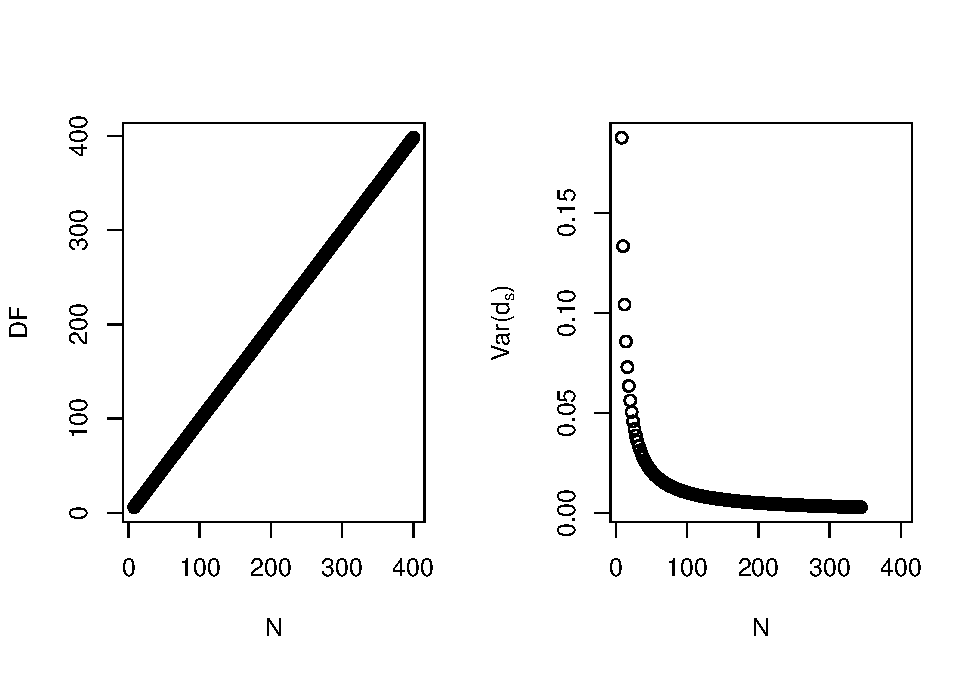
\includegraphics{Theoretical-Variance-of-all-estimators-as-a-function-of-population-parameters_files/figure-latex/varshiehhomNsize2-1.pdf}
\caption{\label{fig:varshiehhomNsize2}Variance of Shieh's \(d_s\) when variances are equal across groups, as a function of the total sample size (N), for a constant sample sizes ratio (\(log\left(\frac{n_1}{n_2} \right)\)).}
\end{figure}

\begin{figure}
\centering
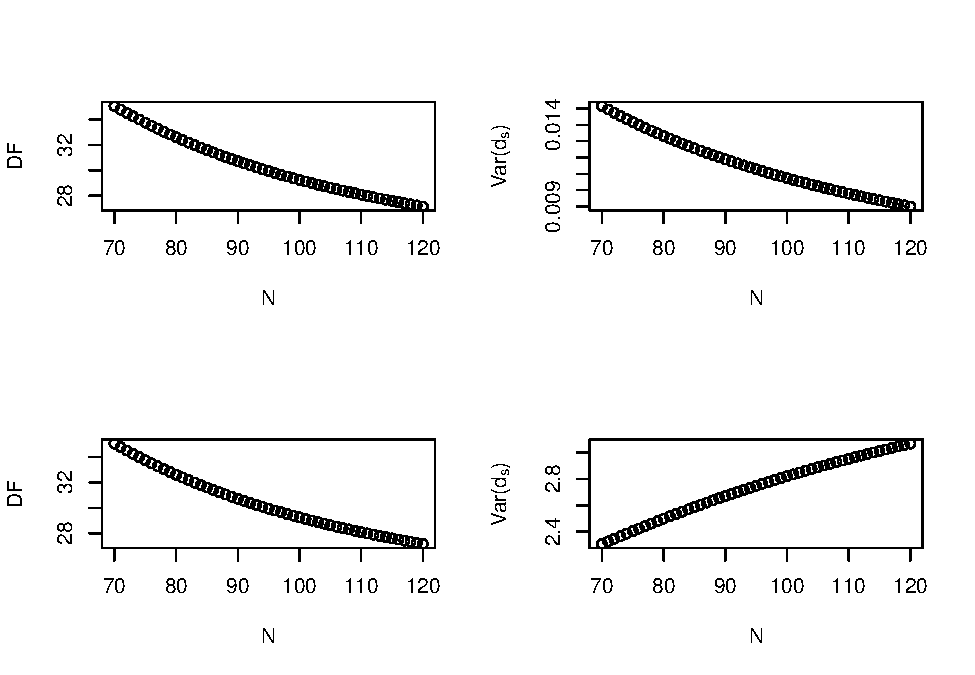
\includegraphics{Theoretical-Variance-of-all-estimators-as-a-function-of-population-parameters_files/figure-latex/varshiehhomNsize4-1.pdf}
\caption{\label{fig:varshiehhomNsize4}Variance of Shieh's \(d_s\) when variances are equal across groups, as a function of the total sample size (N), when adding subjects only in one group (either in the first group; see top plots; or in the second group; see bottom plots).}
\end{figure}

\begin{itemize}
\tightlist
\item
  The larger the total sample size, the lower the variance, whatever the sample sizes ratio is constant (see Figure \ref{fig:varshiehhomNsize2}) or not (see Figure \ref{fig:varshiehhomNsize4}).
\end{itemize}

Note: in \enquote{Theoretical Bias, as a function of population parameters}, we noticed that increasing the sample sizes ratio when adding subjects in only one group could decrease the degrees of freedom. However, due to the \enquote{N} in the denominator of the variance computation, even when degrees of freedom decrease due to the fact that one adds subjects only in one group, the variance still decreases (because the denominator of the variance computation increases; see Figure \ref{fig:varshiehhomNsize4}).

\hypertarget{when-bf-pmbdelta_shieh-neq-0}{%
\paragraph{\texorpdfstring{When \(\bf \pmb{\delta_{Shieh}} \neq 0\)}{When \textbackslash bf \textbackslash pmb\{\textbackslash delta\_\{Shieh\}\} \textbackslash neq 0}}\label{when-bf-pmbdelta_shieh-neq-0}}

While the variance of Shieh's \(d_s\) still depends on the total sample size and the sample sizes ratio, it also depends on the population effect size (\(\delta_{Shieh}\)): the larger the population effect size, the larger the variance. However, the effect of the population effect size decreases when the degrees of freedom increase (i.e.~when sample sizes increase, without increasing the sample sizes ratio, and/or the sample sizes ratio get closer to 1), as previously illustrated in Figure \ref{fig:ESmoderator2}.

Note: we previously noticed that when the effet size is zero, the variance of Shieh's \(d_s\) decreases, even when the sample sizes ratio increases. It is no longer true when there is a non-null effect size because the larger the sample sizes ratio, the more the variance will increase with increasing effect size.

\hypertarget{when-variances-are-unequal-across-populations-with-equal-sample-sizes-2}{%
\subsubsection{When variances are unequal across populations, with equal sample sizes}\label{when-variances-are-unequal-across-populations-with-equal-sample-sizes-2}}

\hypertarget{when-bf-pmbdelta_shieh0-1}{%
\paragraph{\texorpdfstring{When \(\bf \pmb{\delta_{Shieh}}=0\)}{When \textbackslash bf \textbackslash pmb\{\textbackslash delta\_\{Shieh\}\}=0}}\label{when-bf-pmbdelta_shieh0-1}}

When the population effect size is zero, the variance of Shieh's \(d_s\) can be simplified as follows:

\[Var_{Shieh's \; d_s} = \frac{df}{(df-2)N}\]
with \(df = \frac{(\sigma_1^2+\sigma_2^2)^2 \times (n-1)}{\sigma_1^4+\sigma_2^4}\). In this configuration, the degrees of freedom as well as the variance of Shieh's \(d_s\) depend on the total sample size (N) and the \(SD\)-ratio (\(\frac{\sigma_1}{\sigma_2}\)).

\begin{figure}
\centering
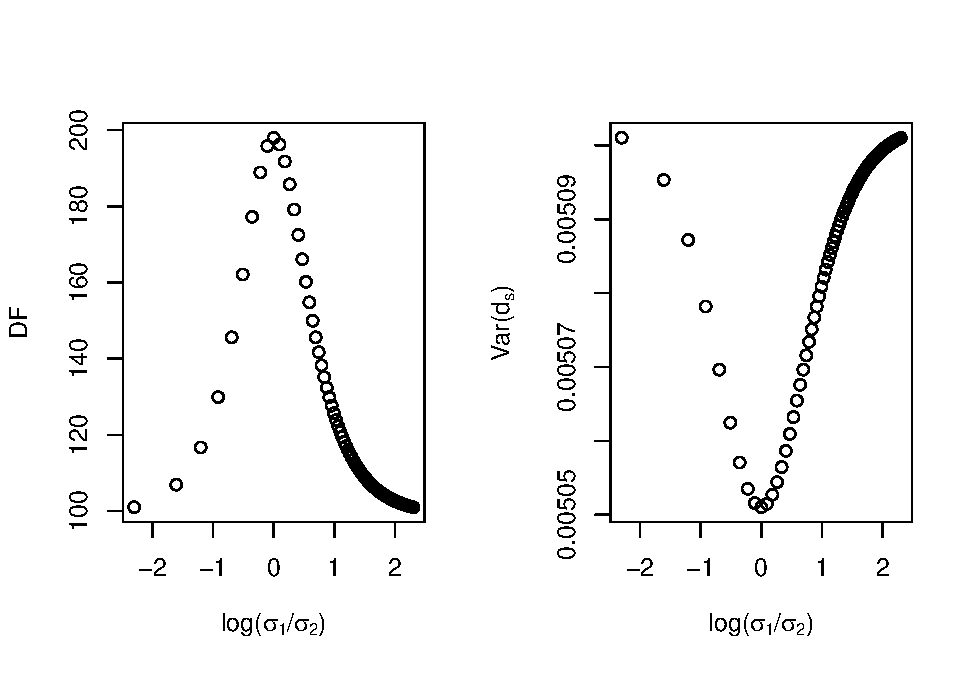
\includegraphics{Theoretical-Variance-of-all-estimators-as-a-function-of-population-parameters_files/figure-latex/varshiehhetbalSDratio2-1.pdf}
\caption{\label{fig:varshiehhetbalSDratio2}Variance of Shieh's \(d_s\) when variances are unequal across groups and sample sizes are equal, as a function of the logarithm of the \(SD\)-ratio (\(log \left( \frac{\sigma_1}{\sigma_2} \right)\)).}
\end{figure}

\begin{itemize}
\tightlist
\item
  The further the SD-ratio is from 1, the larger the variance (see Figure \ref{fig:varshiehhetbalSDratio2});
\end{itemize}

\begin{figure}
\centering
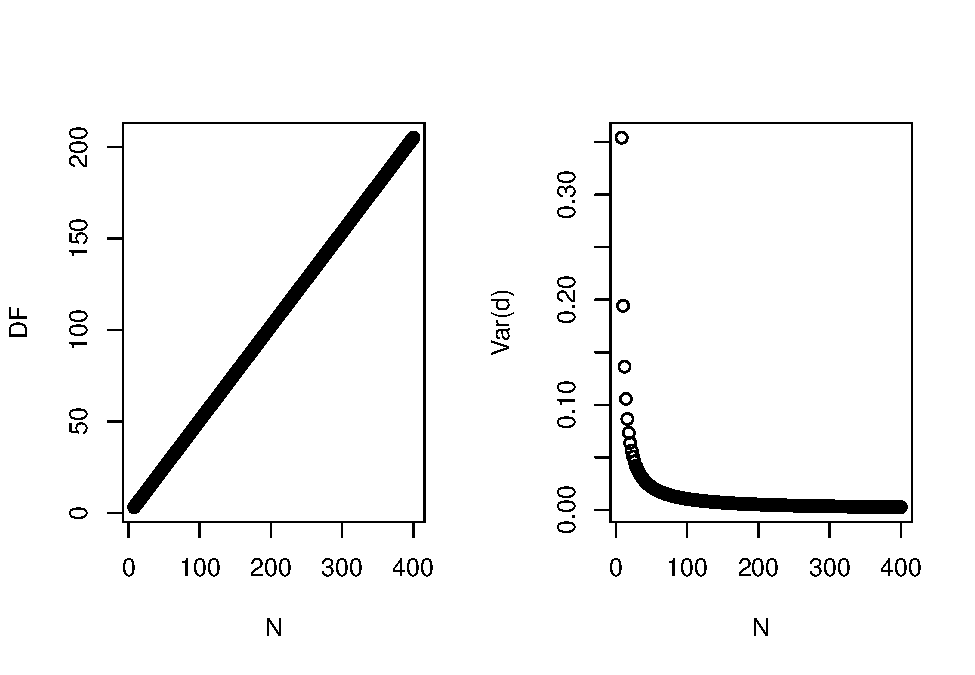
\includegraphics{Theoretical-Variance-of-all-estimators-as-a-function-of-population-parameters_files/figure-latex/varshiehhetbalNsize2-1.pdf}
\caption{\label{fig:varshiehhetbalNsize2}Variance of Cohen's \(d^*_s\) when variances are unequal across groups and sample sizes are equal, as a function of the total sample size (N).}
\end{figure}

\begin{itemize}
\tightlist
\item
  The larger the total sample size, the lower the variance (see Figure \ref{fig:varshiehhetbalNsize2}).
\end{itemize}

\begin{figure}
\centering
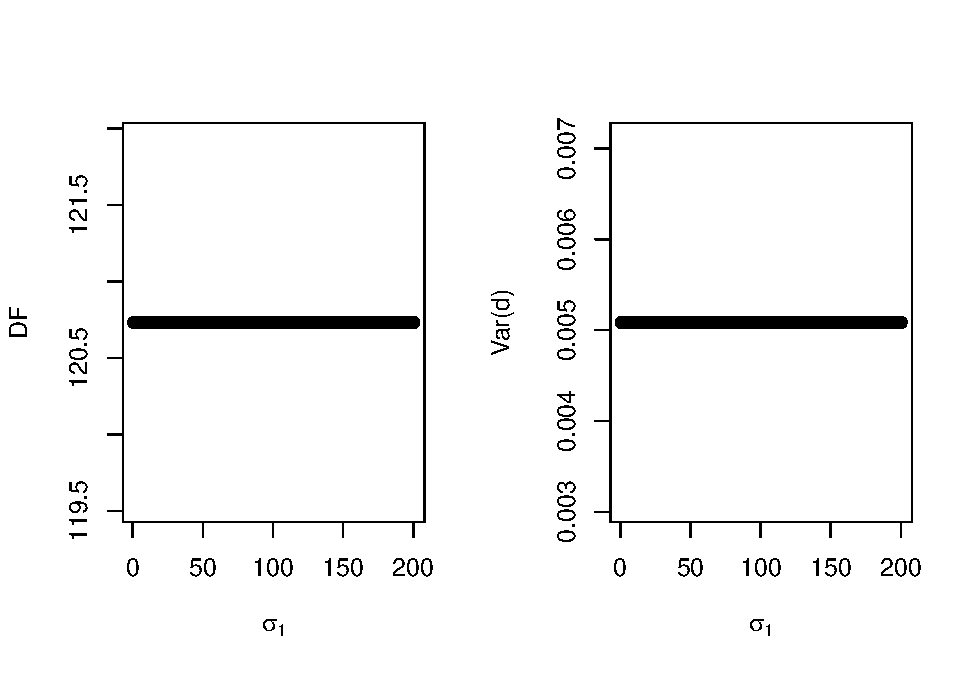
\includegraphics{Theoretical-Variance-of-all-estimators-as-a-function-of-population-parameters_files/figure-latex/varshiehhetbalvariance2-1.pdf}
\caption{\label{fig:varshiehhetbalvariance2}Variance of Shieh's \(d_s\), when variances are unequal across groups and sample sizes are equal, as a function of \(\sigma_1\) and \(\sigma_2\), for a constant \(SD\)-ratio.}
\end{figure}

Note: for a constant SD-ratio, the size of the variance does not matter (see Figure \ref{fig:varshiehhetbalvariance2}).

\hypertarget{when-bf-pmbdelta_shieh-neq-0-1}{%
\paragraph{\texorpdfstring{When \(\bf \pmb{\delta_{Shieh}} \neq 0\)}{When \textbackslash bf \textbackslash pmb\{\textbackslash delta\_\{Shieh\}\} \textbackslash neq 0}}\label{when-bf-pmbdelta_shieh-neq-0-1}}

While the variance of Shieh's \(d_s\) still depends on the total sample size and the \(SD\)-ratio, it also depends on the population effect size (\(\delta_{Shieh}\)): the larger the population effect size, the larger the variance. However, the effect of the population effect size decreases when the degrees of freedom increase (i.e.~when sample sizes increase and/or the \(SD\)-ratio get closer to 1), as previously illustrated in Figure \ref{fig:ESmoderator2}.

\hypertarget{when-variances-are-unequal-across-populations-with-unequal-sample-sizes-2}{%
\subsubsection{When variances are unequal across populations, with unequal sample sizes}\label{when-variances-are-unequal-across-populations-with-unequal-sample-sizes-2}}

\hypertarget{when-bf-pmbdelta_shieh0-2}{%
\paragraph{\texorpdfstring{When \(\bf \pmb{\delta_{Shieh}}=0\)}{When \textbackslash bf \textbackslash pmb\{\textbackslash delta\_\{Shieh\}\}=0}}\label{when-bf-pmbdelta_shieh0-2}}

When the population effect size is zero, the variance of Shieh's \(d_s\) can be simplified as follows:

\[Var_{Shieh's \; d_s} = \frac{df}{(df-2)N}\]
with \(df = \frac{\left(\frac{\sigma^2_1}{n_1}+\frac{\sigma^2_2}{n_2} \right)^2}{\frac{(\sigma^2_1/n_1)^2}{n_1-1}+\frac{(\sigma^2_2/n_2)^2}{n_2-1}}\). In this configuration, the degrees of freedom as well as the variance of Shieh's \(d_s\) depend on the total sample size (\(N\)) and the interaction between the sample sizes ratio and the \(SD\)-ratio \(\left(\frac{n_1}{n_2}\times\frac{\sigma_1}{\sigma_2} \right)\):

\begin{figure}
\centering
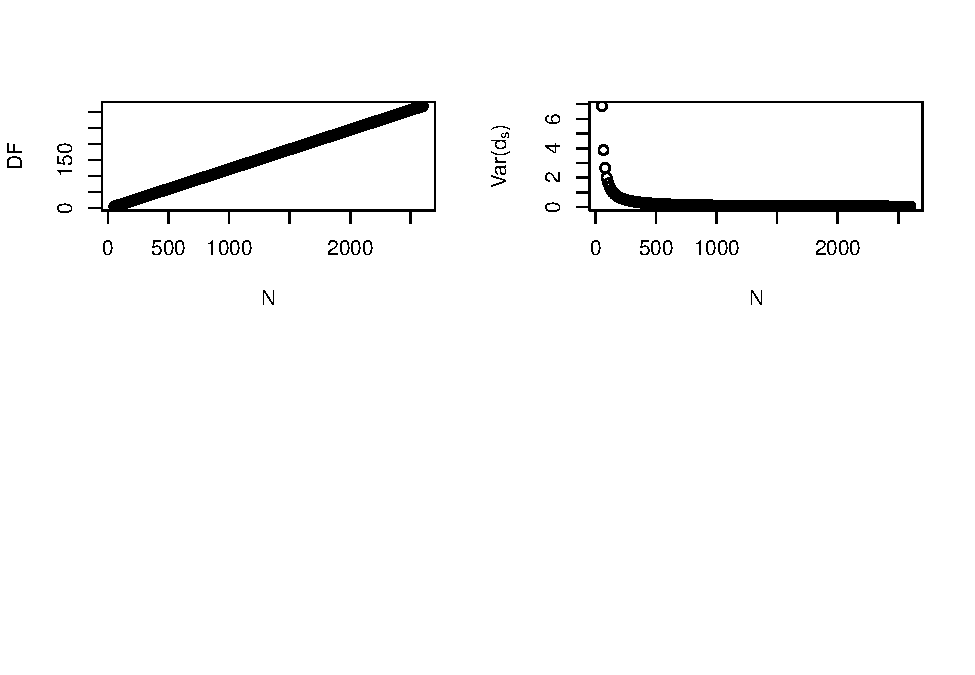
\includegraphics{Theoretical-Variance-of-all-estimators-as-a-function-of-population-parameters_files/figure-latex/varshiehhetunbalNsize2-1.pdf}
\caption{\label{fig:varshiehhetunbalNsize2}Variance of Shieh's \(d_s\) when variances and sample sizes are unequal across groups, as a function of the total sample size (N), for a constant sample sizes ratio (\(log\left(\frac{n_1}{n_2} \right)\)).}
\end{figure}

\begin{figure}
\centering
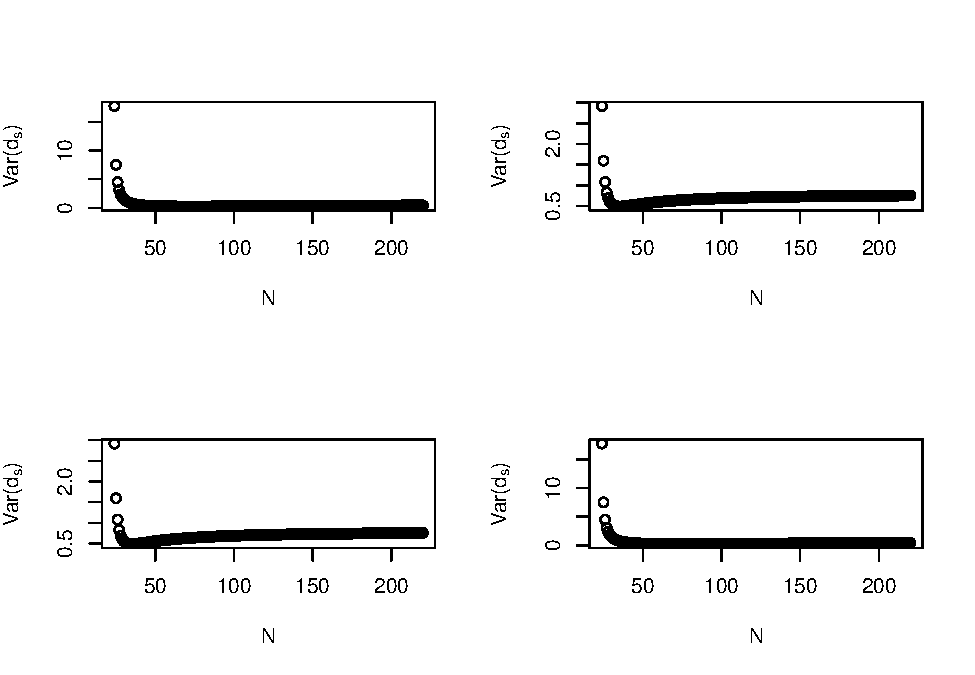
\includegraphics{Theoretical-Variance-of-all-estimators-as-a-function-of-population-parameters_files/figure-latex/varshiehhetunbalNsize4-1.pdf}
\caption{\label{fig:varshiehhetunbalNsize4}Variance of Shieh's \(d_s\) when variances and sample sizes are unequal across groups, as a function of the total sample size (N), when adding subjects only in one group (either in the first group; see left plots; or in the second group; see right plots), and \(\sigma_1 > \sigma_2\) (top plots) or \(\sigma_1 < \sigma_2\) (bottom plots).}
\end{figure}

\begin{itemize}
\tightlist
\item
  The larger the total sample size, the lower the variance, whatever the sample sizes ratio is constant (see Figure \ref{fig:varshiehhetunbalNsize2}) or not (see Figure \ref{fig:varshiehhetunbalNsize4}).
\end{itemize}

Note: When variances were equal across populations, adding subjects only in the first group had the same impact on the variance than adding subjects only in the second group (see Figure \ref{fig:varshiehhomNsize4}). When variances are unequal across groups, this is not true anymore (see Figure \ref{fig:varshiehhetunbalNsize4}).

\begin{figure}
\centering
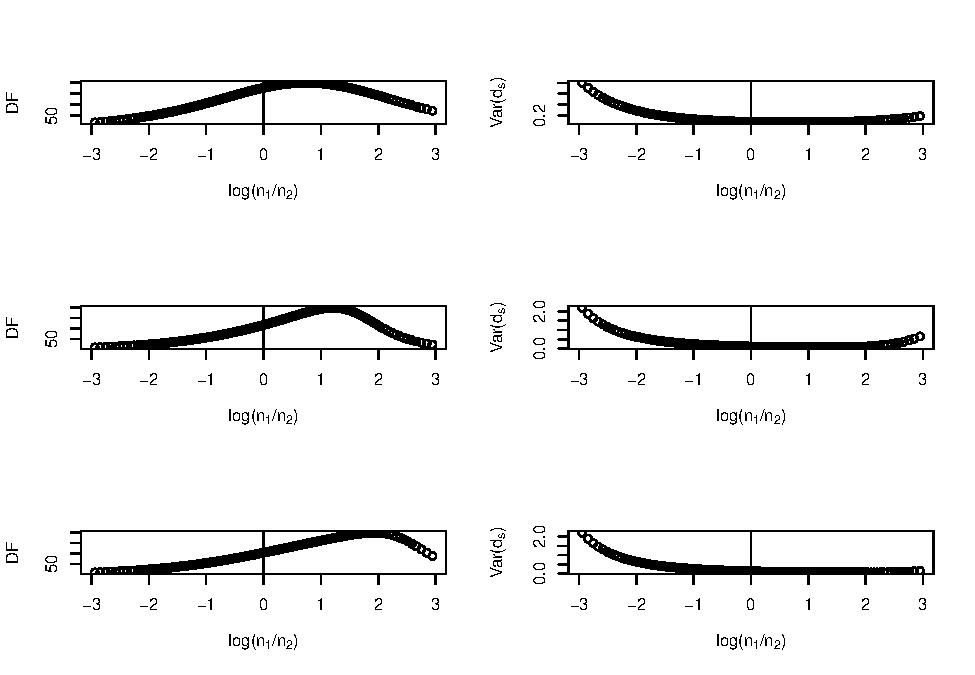
\includegraphics{Theoretical-Variance-of-all-estimators-as-a-function-of-population-parameters_files/figure-latex/varshiehhetunbaldfandvar-1.pdf}
\caption{\label{fig:varshiehhetunbaldfandvar}The variance of Shieh's \(d_s\), when variances and sample sizes are unequal across groups, as a function of the logarithm of the sample sizes ratio (\(log \left( \frac{n_1}{n_2} \right)\)), when \(SD\)-ratio equals 1.46 (first row), 3.39 (second row) or 7 (third row).}
\end{figure}

\begin{itemize}
\tightlist
\item
  The smallest variance always occurs when there is a positive pairing between variances and sample size. Moreover, the further the \(SD\)-ratio is from 1, the further from 1 will also be the sample sizes ratio associated with the smallest var (see Figure \ref{fig:varshiehhetunbaldfandvar}).
\end{itemize}

\begin{figure}
\centering
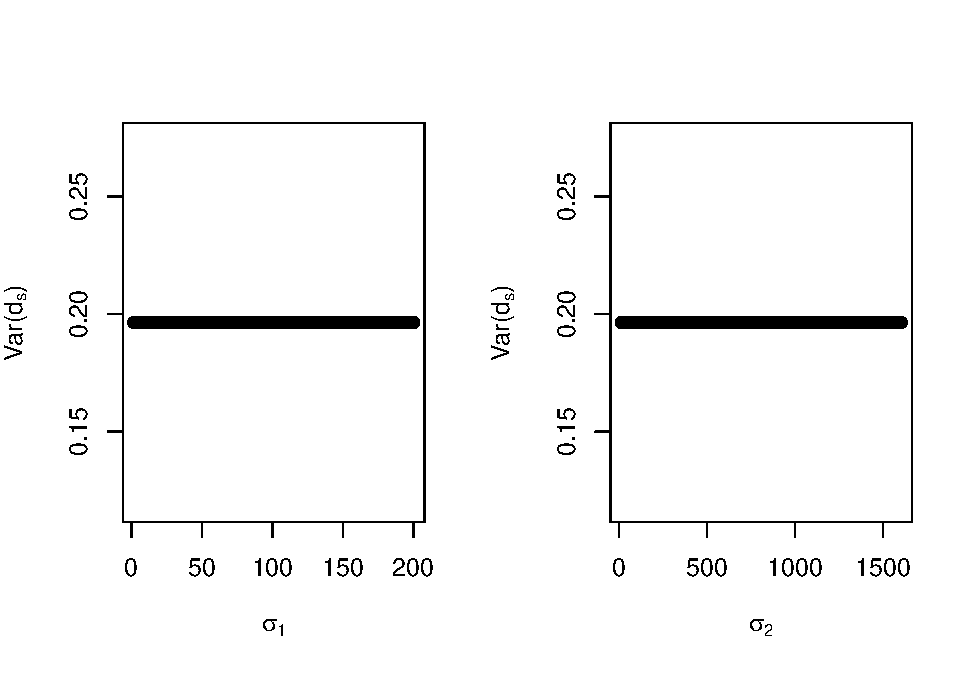
\includegraphics{Theoretical-Variance-of-all-estimators-as-a-function-of-population-parameters_files/figure-latex/varshiehhetunbalvariance2-1.pdf}
\caption{\label{fig:varshiehhetunbalvariance2}Variance of Shieh's \(d_s\), when variances and sample sizes are unequal across groups, as a function of \(\sigma_1\) (left) or \(\sigma_2\) (right), for a constant \(SD\)-ratio.}
\end{figure}

Moreover, for a constant SD-ratio, the variances don't matter (See Figure \ref{fig:varshiehhetunbalvariance2}).

\hypertarget{when-bf-pmbdelta_shieh-neq-0-2}{%
\paragraph{\texorpdfstring{When \(\bf \pmb{\delta_{Shieh}} \neq 0\)}{When \textbackslash bf \textbackslash pmb\{\textbackslash delta\_\{Shieh\}\} \textbackslash neq 0}}\label{when-bf-pmbdelta_shieh-neq-0-2}}

While the variance of Shieh's \(d_s\) still depends on the total sample size and the interaction between the sample sizes ratio and the \(SD\)-ratio, it also depends on the population effect size (\(\delta_{Shieh}\)): the larger the population effect size, the larger the variance. However, the effect of the population effect size decreases when the degrees of freedom increase, as previously illustrated in Figure \ref{fig:ESmoderator2}.

\hypertarget{in-summary-3}{%
\subsubsection{In summary}\label{in-summary-3}}

The variance of Shieh's \(d_s\) is a function of the population effect size (\(\delta_{Shieh}\)), the total sample size (N) and the interaction between sample sizes ratio and \(SD\)-ratio \(\left(\frac{n_1}{n_2}\times\frac{\sigma_1}{\sigma_2} \right)\):

\begin{itemize}
\item
  The variance always decreases when the control and/or the experimental group increases. The benefit of adding subjects rather in the control or in the experimental group depends on the \(SD\)-ratio. Indeed, the smallest variance always occurs when there is a positive pairing between variances and sample sizes. Moreover, the further the \(SD\)-ratio is from 1, the further from 1 will also be the sample sizes ratio associated with the smallest variance;
\item
  The variance increases when \(\delta_{Shieh}\) increases. Note that the effect of \(\delta_{Shieh}\) is moderated by the total sample size and the interaction between the sample sizes ratio and the \(SD\)-ratio.
\end{itemize}


\end{document}
